
\documentclass[10pt,a4paper]{article}
\usepackage{f1000_styles}

%% Default: numerical citations
% \usepackage[numbers]{natbib}

%% Uncomment this lines for superscript citations instead
% \usepackage[super]{natbib}

%% Uncomment these lines for author-year citations instead
% \usepackage[round]{natbib}
% \let\cite\citep

%% lines required to use a CSL style for references
% definitions for citeproc citations
\NewDocumentCommand\citeproctext{}{}
\NewDocumentCommand\citeproc{mm}{%
  \begingroup\def\citeproctext{#2}\cite{#1}\endgroup}
\makeatletter
 % allow citations to break across lines
 \let\@cite@ofmt\@firstofone
 % avoid brackets around text for \cite:
 \def\@biblabel#1{}
 \def\@cite#1#2{{#1\if@tempswa , #2\fi}}
\makeatother
\newlength{\cslhangindent}
\setlength{\cslhangindent}{1.5em}
\newlength{\csllabelwidth}
\setlength{\csllabelwidth}{3em}
\newenvironment{CSLReferences}[2] % #1 hanging-indent, #2 entry-spacing
 {\begin{list}{}{%
  \setlength{\itemindent}{0pt}
  \setlength{\leftmargin}{0pt}
  \setlength{\parsep}{0pt}
  % turn on hanging indent if param 1 is 1
  \ifodd #1
   \setlength{\leftmargin}{\cslhangindent}
   \setlength{\itemindent}{-1\cslhangindent}
  \fi
  % set entry spacing
  \setlength{\itemsep}{#2\baselineskip}}}
 {\end{list}}
\usepackage{calc}
\newcommand{\CSLBlock}[1]{\hfill\break#1\hfill\break}
\newcommand{\CSLLeftMargin}[1]{\parbox[t]{\csllabelwidth}{\strut#1\strut}}
\newcommand{\CSLRightInline}[1]{\parbox[t]{\linewidth - \csllabelwidth}{\strut#1\strut}}
\newcommand{\CSLIndent}[1]{\hspace{\cslhangindent}#1}

%% lines to get the code chunks working

%% lines to enable bulletpoints in a new notation style
\providecommand{\tightlist}{%
  \setlength{\itemsep}{0pt}\setlength{\parskip}{0pt}}

\begin{document}
\pagestyle{fancy}

\title{The Biogeography of Morphological Variation in Corvus macrorhynchos}
\author[1]{Aubrey Lynn Alamshah*}
\author[2]{Benjamin Michael Marshall}
\affil[1]{Department of Biological Sciences, Binghamton University, Binghamton, NY, USA}
\affil[2]{School of Biodiversity, One Health and Veterinary Medicine, University of Glasgow, Glasgow, UK}
\affil[*]{\href{mailto:aubrey.alamshah@gmail.com}{\nolinkurl{aubrey.alamshah@gmail.com}}}

\maketitle
\thispagestyle{fancy}

\begin{abstract}

Examinations of morphology can reveal a species' relationship with the environment and their evolutionary trajectory. Particularly pronounced difference can hint at specific selection pressures, and reveal hitherto unknown species. Cryptic species, with only subtle morphological differences, are widespread and ignoring them risks underestimating biodiversity and their threatened status. Recently several prominent examples of splits of widespread species complex have occurred in Asia. We turned our attention to the Jungle Crow (\emph{Corvus macrorhynchos}), who has been the subject of taxonomic debate for over a century. Using museums specimens, sourced from across their distribution, we used standardised photography to measured the hard tissue morphology of over 1,000 \emph{Corvus macrorhynchos}. We examined how these hard tissue measures compared to two previously proposed subspecies delineations. We revealed that most boundaries are not visible in the hard tissue measures, with \emph{Corvus macrorhynchos phillipinus} being a notable exception. In general, hard tissues only exhibit small differences across the distribution. However, spatial exploration of these data highlighted several areas exhibited unique morphology, namely Japan, Northern India, and the Philippines. We explored several climatic explanations for these patterns, which highlighted a potential association between temperature and the form of the bill. The limited variation may be suggest that Jungle Crows are adapting locally and flexibly through behaviour, rather than via major morphological change. Therefore, subspecies definitions may be more visible in other phenotypic traits, or only detectable via genetic methods. The conspicuous morphology of \emph{Corvus macrorhynchos} Japan, Northern India, and the Philippines warrants further comparative investigation to determine potential drivers.

\end{abstract}

\section*{Keywords}

jungle crow, Corvus macrorhynchos, morphology, biogeography, species complex, museum specimens, Corvidae

\clearpage
\pagestyle{fancy}

\section{Introduction}\label{introduction}

Examining morphology can help us pinpoint particular selection pressures on a species.
Environmental drivers such as climate often produce morphological responses (\citeproc{ref-ashton_patterns_2002}{Ashton, 2002}).
Behaviour can both limit morphological changes by providing a way to adapt without having to physically change (\citeproc{ref-huey_behavioral_2003}{Huey, Hertz \& Sinervo, 2003}), or drive changes itself by enabling the exploitation of new niches (\citeproc{ref-wyles_birds_1983}{Wyles, Kunkel \& Wilson, 1983}).
Observing the morphological variation, or lack thereof, in a species that occupies a wide gradient of environmental variation will aid identification of the relative importance of behaviour and morphology in adaptation.
Crows and ravens (Genus \emph{Corvus}) exist across many different environments in their distribution across the globe, both as a group and generally within \emph{Corvus} species (\citeproc{ref-madge_crows_1999}{Madge \& Burn, 1999}).
For example, 23 out of the 44 extant species within \emph{Corvus} would be considered ``generalists'' and have large distributions across multiple habitat types (\citeproc{ref-iucn_corvus_2016}{IUCN, 2016}).
One could expect a crow species spread across a wide area to have a wide range of morphological adaptations to tackle this diversity of environments.
However, \emph{Corvus} species are famously behaviourally adaptable, presenting an opportunity to reduce environmental pressure without the need for morphological changes (\citeproc{ref-sol_behavioural_2002}{Sol, Timmermans \& Lefebvre, 2002}).
This survival through behavioural flexibility may help to explain the lack of phenotypic diversity across the \emph{Corvus} genus.

In instances where morphology does differ in \emph{Corvus}, it has provided insight into how behaviour can drive morphological adaptations.
For example, New Caledonian Crows have a bill shape that enhances their ability to make and use tools.
The presence of such a unique morphological character allows us to infer the importance of tool use in New Caledonian Crows' survival (\citeproc{ref-troscianko_extreme_2012}{Troscianko et al., 2012}; \citeproc{ref-rutz_evolutionary_2012}{Rutz \& St Clair, 2012}).
New Caledonian Crows live in an isolated, relatively homogeneous island environment with limited mobility, population size and foraging options, that have probably enhanced the selection pressure for more efficient foraging.
Examining a more widely distributed and mobile crow that lives across a diversity of environments may offer a more typical scenario encompassing the interplay of behaviour, environment, and morphology in \emph{Corvus spp.}
The Jungle Crow (\emph{Corvus macrorhynchos}) is one of the most widely distributed crow species, ranging from Russia in the north to Indonesia in the south, from Afghanistan in the west to the Japan in the East.
The presence of geographical patterns of morphological variation in \emph{C. macrorhynchos} has been noted for nearly a century (\citeproc{ref-hartert_types_1922}{Hartert \& Zoological Museum (Tring, England), 1922}), but these descriptions do not include the full species range.
The presence of areas of divergence does seem likely given the shared bio-geographical barriers seen in other widely distributed Asian species, particularly between islands and the mainland, as well as across the drastic elevation changes in the Himalayas (\citeproc{ref-garg_genome-wide_2016}{Garg et al., 2016}; \citeproc{ref-gwee_species_2019}{Gwee et al., 2019}; \citeproc{ref-singh_taxonomy_2020}{Singh et al., 2020}).
Several studies, reinforced by field guides, already suggest that \emph{C. macrorhynchos} differ significantly in morphology on regional scales (\citeproc{ref-dickinson_systematic_2004}{Dickinson, Eck \& Martens, 2004}; \citeproc{ref-madge_crows_2010}{Madge \& Burn, 2010}; \citeproc{ref-nakamura_postglacial_2016}{Nakamura \& Kryukov, 2016}) and several species or subspecies divisions have been proposed (\citeproc{ref-klockenhoff_zur_1969}{Klockenhoff, 1969}; \citeproc{ref-martens_calls_2000}{Martens, 2000}).
Until now, however, a rigorous distribution-wide investigation has yet to be conducted and presents the opportunity to highlight macro-patterns of morphological variation in relation to the species' full range of geography and climate.
So far, the most comprehensive taxonomic examinations of \emph{C. macrorhynchos} have not analysed morphological variation but used feather parasites (\citeproc{ref-klockenhoff_zur_1969}{Klockenhoff, 1969}) and vocalizations (\citeproc{ref-martens_calls_2000}{Martens, 2000}).
Both reports refer to \emph{C. macrorhynchos} as a species complex, but Klockenhoff (\citeproc{ref-klockenhoff_zur_1969}{1969}) proposes 12 distinct subspecies with three areas of hybridization of which seven are mainland subspecies and five island subspecies (Fig. \ref{fig:subspeciesPlots}.
These subspecies were defined by the biogeographic boundaries of mallophagan feather parasites (genus \emph{Myrsidea}) that live on \emph{C. macrorhynchos}, as opposed to any characteristics of the birds themselves.
Martens (\citeproc{ref-martens_calls_2000}{2000}) suggests four full species (Fig. \ref{fig:subspeciesPlots}, heavily relying on Klockenhoff's original boundaries as well as personal observations in the Himalayas (\citeproc{ref-martens_towards_1995}{Martens \& Eck, 1995}) where vocal sampling was deficient (Figure 2-1).
Martens (\citeproc{ref-martens_calls_2000}{2000}) groups several island and mainland populations that Klockenhoff (\citeproc{ref-klockenhoff_zur_1969}{1969}) separated, but \emph{C. macrorhynchos} in the Philippines remain separated in both proposals.
In neither study was sampling effort high enough to cover the entire distributions, nor were the parasite or vocal patterns connected with morphological variation or explicit ecological factors.
Neither of these studies have been corroborated by genetic studies, so population or species-level delineation in this group remains unresolved.
(Note: Although Martens (\citeproc{ref-martens_calls_2000}{2000}) suggests species-level divisions, we will refer to both proposed groupings as subspecies for simplicity.)

Many specimens of \emph{C. macrorhynchos} from across the species' distribution exist collectively in museums, presenting an opportunity for a more comprehensive examination of preserved morphological variation in relation to the proposals of population delineation based on feather parasite or vocalization, as well as the ability to relate morphological/behavioural variation to ecological variation.
Furthermore, by covering the entire distribution of \emph{C. macrorhynchos}, such a comprehensive morphological data set can potentially suggest behavioural variation (e.g., in foraging) and serve as a foundation for identifying biogeographical patterns in a way that previous studies could not.
Museum specimens best preserve the ``hard'' morphology of birds, specifically bills and legs.
The bill and tarsal morphology of \emph{C. macrorhynchos} are of particular interest due to their direct interactions with both the environment and behaviour.
Tarsus length can be used as a proxy for body size (\citeproc{ref-senar_keel_1997}{Senar \& Pascual, 1997}) and present one possible adaptation to varying temperature (\citeproc{ref-ashton_patterns_2002}{Ashton, 2002}).
\emph{C. macrorhynchos} range from seasonally cold areas in the Amur region and high-altitude Himalayas, to the consistently hot equatorial regions of Southern India and Indonesia.
The bill size and shape could offer an alternative or complimentary adaptation to temperature, aiding in heat transfer or providing a buffer to protect against heat loss in cold air (\citeproc{ref-geist_nasal_2000}{Geist, 2000}; \citeproc{ref-probst_effects_2022}{Probst, Ralston \& Bentley, 2022}).
Beyond temperature, the bill presents the primary means through which crows interact with the world, functioning in foraging, vocalizing and object manipulation.
The diverse array of environments in which these crows currently exist, from urban and agricultural land to primary forest, rocky coastline, and tropical islands, suggests a whole suite of varying selection pressures on bill shape and size.
Hard tissue measures present an accessible opportunity to view the realized impact of the environment and the crows' interactions with it through their morphology.
Here we report a study of morphological variation of museum specimens representing the whole of \emph{C. macrorhynchos'} distribution.

Our objectives were as follows:

\begin{itemize}
\item
  To compare geographic variation in bill and tarsus measurements from museum specimens across the subspecies divisions previously proposed by Klockenhoff (\citeproc{ref-klockenhoff_zur_1969}{1969}) and Martens (\citeproc{ref-martens_calls_2000}{2000}).
  We predict that we will find morphological differences between populations on the Philippines and those on the mainland, as both proposals separate this population, and one genetic study supports this (\citeproc{ref-jonsson_brains_2012}{Jønsson, Fabre \& Irestedt, 2012}).
  Aside from this population, we predict that there is likely to be significant overlap in morphometrics between proposed subspecies.
\item
  To use these measurements to identify biogeographic trends in morphology, focusing on outlying areas where crows may have a unique combination of morphological traits.
  Once again, we predict that there will be an area of unique morphology in the Philippines and possibly other islands far from the mainland, but that over most of the \emph{C. macrorhynchos'} distribution, measurements will be similar.
\item
  To investigate whether these areas of morphological interest correlate with broad bioclimatic variables such as temperature, seasonality, and precipitation.
  We predict that \emph{C. macrorhynchos} is likely to follow Bergmann's rule, with measurements increasing as temperatures decrease (\citeproc{ref-ashton_patterns_2002}{Ashton, 2002}).
  Combined, these results highlight the variation present in \emph{C. macrorhynchos} morphology that may be indicative of their adaptation to the environment and evolutionary history.
\end{itemize}

\section{Methods}\label{methods}

We used previously published data from Alamshah \& Marshall (\citeproc{ref-alamshah_distribution-wide_2025}{2025}).
Briefly this dataset comprised measures of hard tissue morphology of \emph{Corvus macrorhynchos} from across their distribution.
The sample was based on all available specimens of \emph{C. macrorhynchos} in the American Museum of Natural History (AMNH), Cornell University Museum of Vertebrates (CUMV), Field Museum of Natural History (FMNH), Natural History Museum (NHMUK), and the Smithsonian National Museum of Natural History (USNM).
The protocol for taking measurements involved the taking of a standardised set of photographs; namely four surrounding the head, and two focused on the legs/feet.
The use of photograph in measuring bird morphometrics was previously demonstrated as by (\citeproc{ref-williams_photography_2020}{Williams, Wilcox \& Patterson, 2020}); their standardised procedure for photographing live birds was more or equally as repeatable as calipers measurements.
All the photographs contained standardised reference scales (i.e., background grid or ruler) that enabled digital measures to be collected using imageJ (\citeproc{ref-schneider_nih_2012}{Schneider, Rasband \& Eliceiri, 2012}).
Individuals with damage, fixed in positions that prohibited clear photographs, or demonstrated clear juvenile characteristics (i.e., grey chest feathers, short tail, pink surrounding mouth), were excluded.

Overall the Alamshah \& Marshall (\citeproc{ref-alamshah_distribution-wide_2025}{2025}) dataset contained measurements from 1069 crows total (crows per museum: AMNH: 229, CUMV: 1, FMNH: 118, NHMUK: 550, USNM: 171) measuring Tarsus Length, Bill Base Width, Bill Base Length, Bill Width at Skin Border, Width at Nares, Exposed Culmen, Height at Nares, and Nares to Bill Tip.
We also created created four composite measures: Height at Nares / Tarsus Length, Exposed Culmen / Tarsus Length, Nares to Bill Tip / Exposed Culmen, and Proximal Bill Surface Area.

Height at Nares / Tarsus Length and Exposed Culmen / Tarsus Length represented an estimation of bill height, and exposed culmen length to body size (represented by tarsus length).
The Nares to Bill Tip / Exposed Culmen ratio represented the relative distance of the nares from the bill tip in relation to the bill length as a whole.
A higher number meant that the nares were positioned more proximally on the bill (towards the forehead), and a lower number meant that they were positioned farther distally on the bill (towards the tip).
The Proximal Bill Surface Area was calculated using the following equation: (Exposed Culmen -- Nares to Bill Tip) * Height at Nares / Tarsus Length and it represents an approximation of the surface area of the bill between the nares and the forehead, controlled for body size.
This is an area thought to be important for thermoregulation (\citeproc{ref-tattersall_heat_2009}{Tattersall, Andrade \& Abe, 2009}).

\subsection{Analysis}\label{analysis}

In order to explore how patterns of morphological variation in the dataset corresponded to the proposed subspecies divisions of Klockenhoff (\citeproc{ref-klockenhoff_zur_1969}{1969}), and Martens (\citeproc{ref-martens_calls_2000}{2000}), we took their maps (Figures 2 and 4 in the respective papers) and used QGIS' georeferencing function to convert the figure images to geospatial polygons (\citeproc{ref-QGIS_software}{QGIS Development Team, 2024}).
For Klockenhoff's map, we used coastal and inland landmarks as georeferences; for Martens et al.'s map, we used the provided latitude and longitude scales.
Using the geospatial polygons created from these maps, we then assigned two subspecies identities (one by Klockenhoff's divisions, one by Martens' divisions) to our measured specimens by comparing latitude and longitude locations.

We used a suite of Bayesian models to examine whether the group assignment (subspecies as identified by Klockenhoff or Martens et al.~and sex) could predict the values derived from the photographs and the four ratios based on combined measures.
The models had the formula: \(\mu\) \textasciitilde{} 0 + group:sex, \(\sigma\) \textasciitilde{} 0 + group:sex
Where \(\mu\) is the mean measure, \(\sigma\) is the variance of the measure, group is defined by subspecies and sex is the sex of the crow as identified by the museum metadata.
This allows for a different effect of sex between groups.
All of the models used the Student distribution to reduce the influence of outliers.

There is very little morphometric data for \emph{C. macrorhynchos} at the subspecies level in the published literature, and therefore we relied on broadly defined population-level priors for each measure during parametrisation of the Bayesian models.
Our use of population priors with wide standard deviations means that our estimates of subspecies differences are likely to be conservative, as we had limited options to integrate past knowledge.
We created priors for measures for Width at Nares (WN) (17mm), Height at Nares (22mm), total Exposed Culmen (62mm), Nares to Bill Tip (42mm) and Tarsus Length (57mm) by averaging the corresponding bill measurements provided by AVONET for \emph{C. macrorhynchos} (\citeproc{ref-tobias_avonet_2022}{Tobias et al., 2022}) and using those means as centres for normal priors with wide (20) standard deviations.
We set all priors to have a lower bound of 0.
For measures without prior data, we used the default uninformative priors generated by the \emph{brms} package (\citeproc{ref-burkner_brms_2017}{Bürkner, 2017a}, \citeproc{ref-burkner_brms_2018}{2018a}, \citeproc{ref-burkner_brms_2021}{2021a}).

We ran a total of 24 Bayesian Regression Models, one for each combination of group (subspecies model, sex) and measure (each morphological measure and the 4 composite measures).
We used the \emph{brms} package to run the models, with the following settings: 1000 iterations, 200 warm-up, 4 chains, and 2 thinning factor.

To diagnose whether the models had adequately converged, we examined R-hat values (checking they were near 1), autocorrelation function plots, and trace plots.
To report performance, we calculated \emph{R\textsuperscript{2}} values, and plotted Posterior Predictive Check plots.
Once the models were complete and we extracted the posterior predictive distributions, we calculated all pair-wise contrasts between groups.
We used these resulting contrast distributions to examine the degree of difference between proposed subspecies.
For plotting purposes, we selected the 95\% highest density credible interval around the median (HDCI).

After assessing the predictability of Klockenhoff and Martens et al.'s proposed subspecies delineations, we looked for spatial patterns in the morphometric measures themselves.
As the measures were only collected at defined geographic points and sampling was not systematic, we elected to use Inverse Distance Weighting (IDW) to estimate the measures as if there was continuous variation between sampled locations.
This allowed us to generate smoothed heat maps for each measure over the crows' distribution and reveal areas with consistently high or low measures.
We used mean square error to select the optimal power of distance for the IDW calculations, exploring values of 0.001, 0.01, and 10.
We allowed a different optimal power to be selected per measure.

\subsection{Climate Comparison}\label{climate-comparison}

To explore the relationship between our morphological measurements and climate factors across \emph{C. macrorhynchos'} distribution, we plotted the specimen collection locations and their associated measurements against maps of mean annual temperature, temperature seasonality, and annual precipitation provided by the CMCC-BioClimInd dataset (\citeproc{ref-noce_cmcc-bioclimind_2019}{Noce, Caporaso \& Santini, 2019}, \citeproc{ref-noce_new_2020}{2020}).
This dataset was developed from global bioclimatic data collected from 1960--1999.
Mean annual temperature refers to the annual average of daily mean temperature, averaged across all years in the collected time period.
Temperature seasonality refers to the temperature change throughout the year; using the average daily mean temperature for each month, it is quantified as the standard deviation among the monthly values.
Higher standard deviation values mean greater seasonal variability.
Annual precipitation refers to the annual sum of daily precipitation averaged along all years within the time period.
We then ran an additional 12 Bayesian Regression Models to examine the relationship between each measure and our chosen three climatic variables, and applied the same model diagnostic methods as the sub-species comparison models.
We ran these models with 2000 iterations, a warm-up of 500, 4 chains, and a thinning factor of 1.

\section{Results}\label{results}

We obtained measurements from 1069 \emph{Corvus macrorhynchos} (crows per museum: AMNH: 229, CUMV: 1, FMNH: 118, NHMUK: 550, USNM: 171).
We could not obtain all measurements from every crow due to specimen positioning (Fig. \ref{fig:overallPlot}), but for all measures we obtained a sample size of over 1000.
Standard deviation (SD) tends to increase with magnitude of measure: with exposed culmen demonstrating the largest spread of values, and bill width at skin border demonstrating the smallest mean and SD (Fig. \ref{fig:overallPlot}).

\begin{figure}
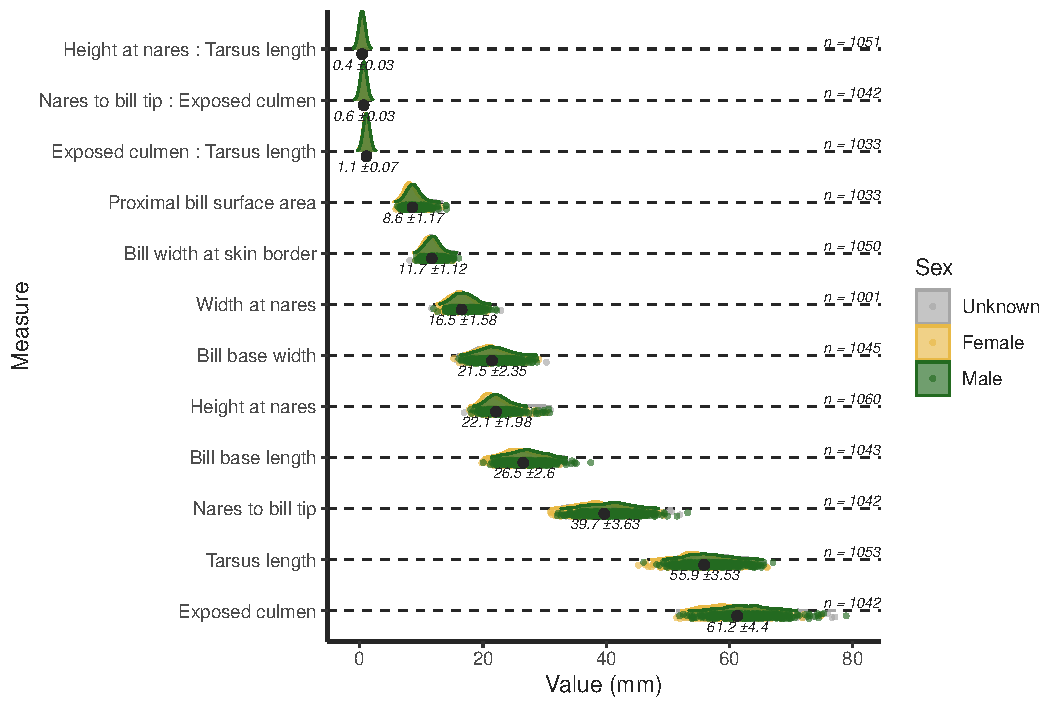
\includegraphics[width=0.9\linewidth]{../Figures/OverallSummaryPlot} \caption{The overall distribution of measurements taken, split between the sexes. Mean and standard deviation labelled below each distribution.}\label{fig:overallPlot}
\end{figure}

The distribution for each sex overlaps heavily regardless of measure, with females showing a tendency to be negligibly smaller on average.
This lack of difference is reflected in the Bayesian Regression Model, where the resulting distributions of contrasts entirely overlap and are largely centred on zero (Fig. \ref{fig:sexContrasts}).
The contrasts suggest a lack of sexual dimorphism in these measures when examined on an overall species level.

The only exceptions exist in Klockenhoff's definition of \emph{C. m. culminatus}, \emph{C. m. hainanus}, and the hybrid zones \emph{lev. x mac.} and \emph{tib. x lev.} (Fig. \ref{fig:sexKlockContrasts}).
\emph{C. m. culminatus} -4.42mm, 95\% HDCI -11.5 to 2.63, 89.53\%, \emph{hainanus} -5.31mm, 95\% HDCI -13.51 to 2.84, 91.21\%, and \emph{levaillantii x macrorhynchos} saw differences in exposed culmen, whereas \emph{levaillantii x tibetosinensis} only showed a difference in bill base length .
\emph{C. m. hainanus} additionally showed a difference in height at nares -5.31mm, 95\% HDCI -13.51 to 2.84, 91.21\%.
All suggesting that females tend to be smaller in these measures.

On an intra-group level, Klockenhoff's groupings also showed little difference between sexes for the majority of measures.
The only exceptions exist in Klockenhoff's definition of \emph{C. m. culminatus}, \emph{C. m. hainanus}, and the hybrid zones \emph{levaillantii} x \emph{macrorhynchos} and \emph{tibetosinensis} x \emph{levaillantii} (Fig. \ref{fig:sexKlockContrasts}).

\emph{Corvus macrorhynchos culminatus}, \emph{hainanus} and \emph{levaillantii} x \emph{macrorhynchos} showed differences in Exposed Culmen, whereas \emph{levaillantii} x \emph{tibetosinensis} only showed a difference in Bill Base Length.
\emph{Corvus macrorhynchos hainanus} additionally showed a difference in Height at Nares.
All of these suggest that females tend to be smaller in these measures.

Martens et al's groupings showed very little difference between sexes (Fig. \ref{fig:sexMartensContrasts}).

We plotted the locations of the specimens against the proposed subspecies maps of Klockenhoff and of Martens et al., allowing us to assign each specimen a subspecies under each proposition.
Our sample of specimens included representatives from all proposed groupings from both studies (Fig. \ref{fig:subspeciesPlots}).

\begin{figure}
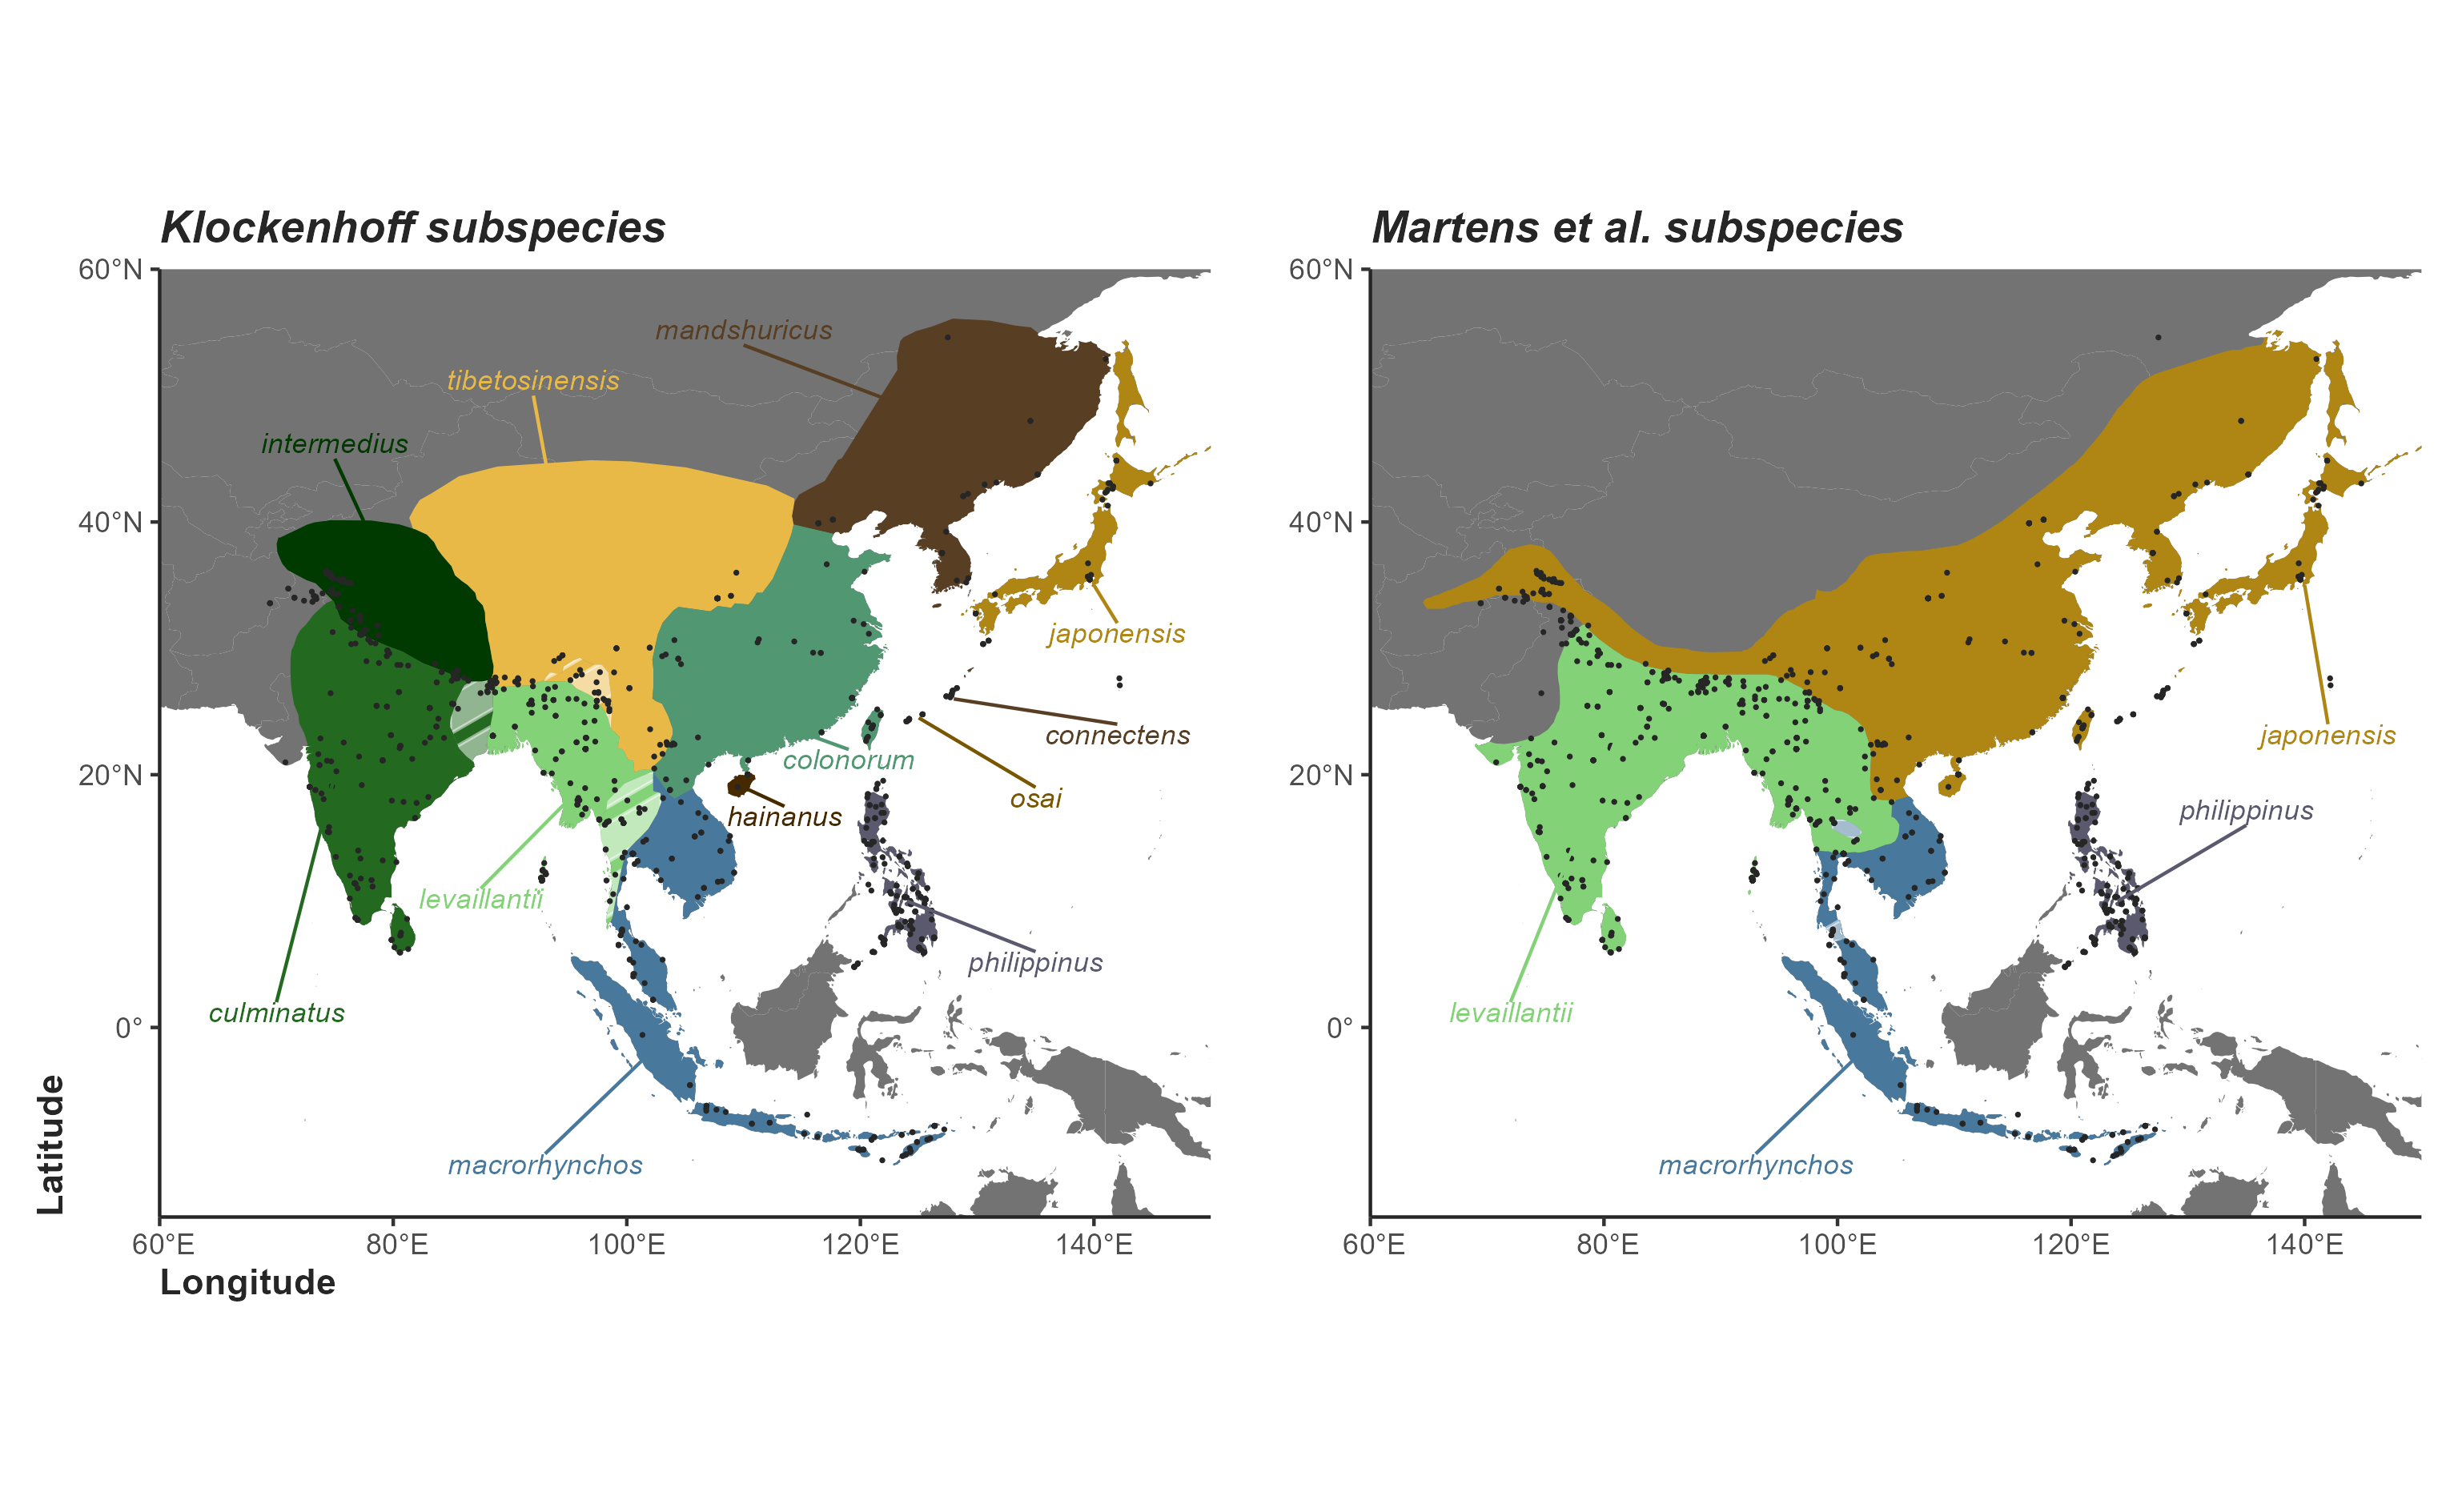
\includegraphics[width=0.9\linewidth]{../Figures/combined Subspecies Plot} \caption{The locations of origin for all museum specimens[.] measured in this study plotted on the proposed subspecies separations from a) Klockenhoff (1969) and b) Martens (2000). Klockenhoff described 12 subspecies and 3 hybrid zones (denoted by the lighter shaded colours). Martens described 4 subspecies and two hybrid zones denoted by the grey shaded areas.}\label{fig:subspeciesPlots}
\end{figure}

\begin{figure}
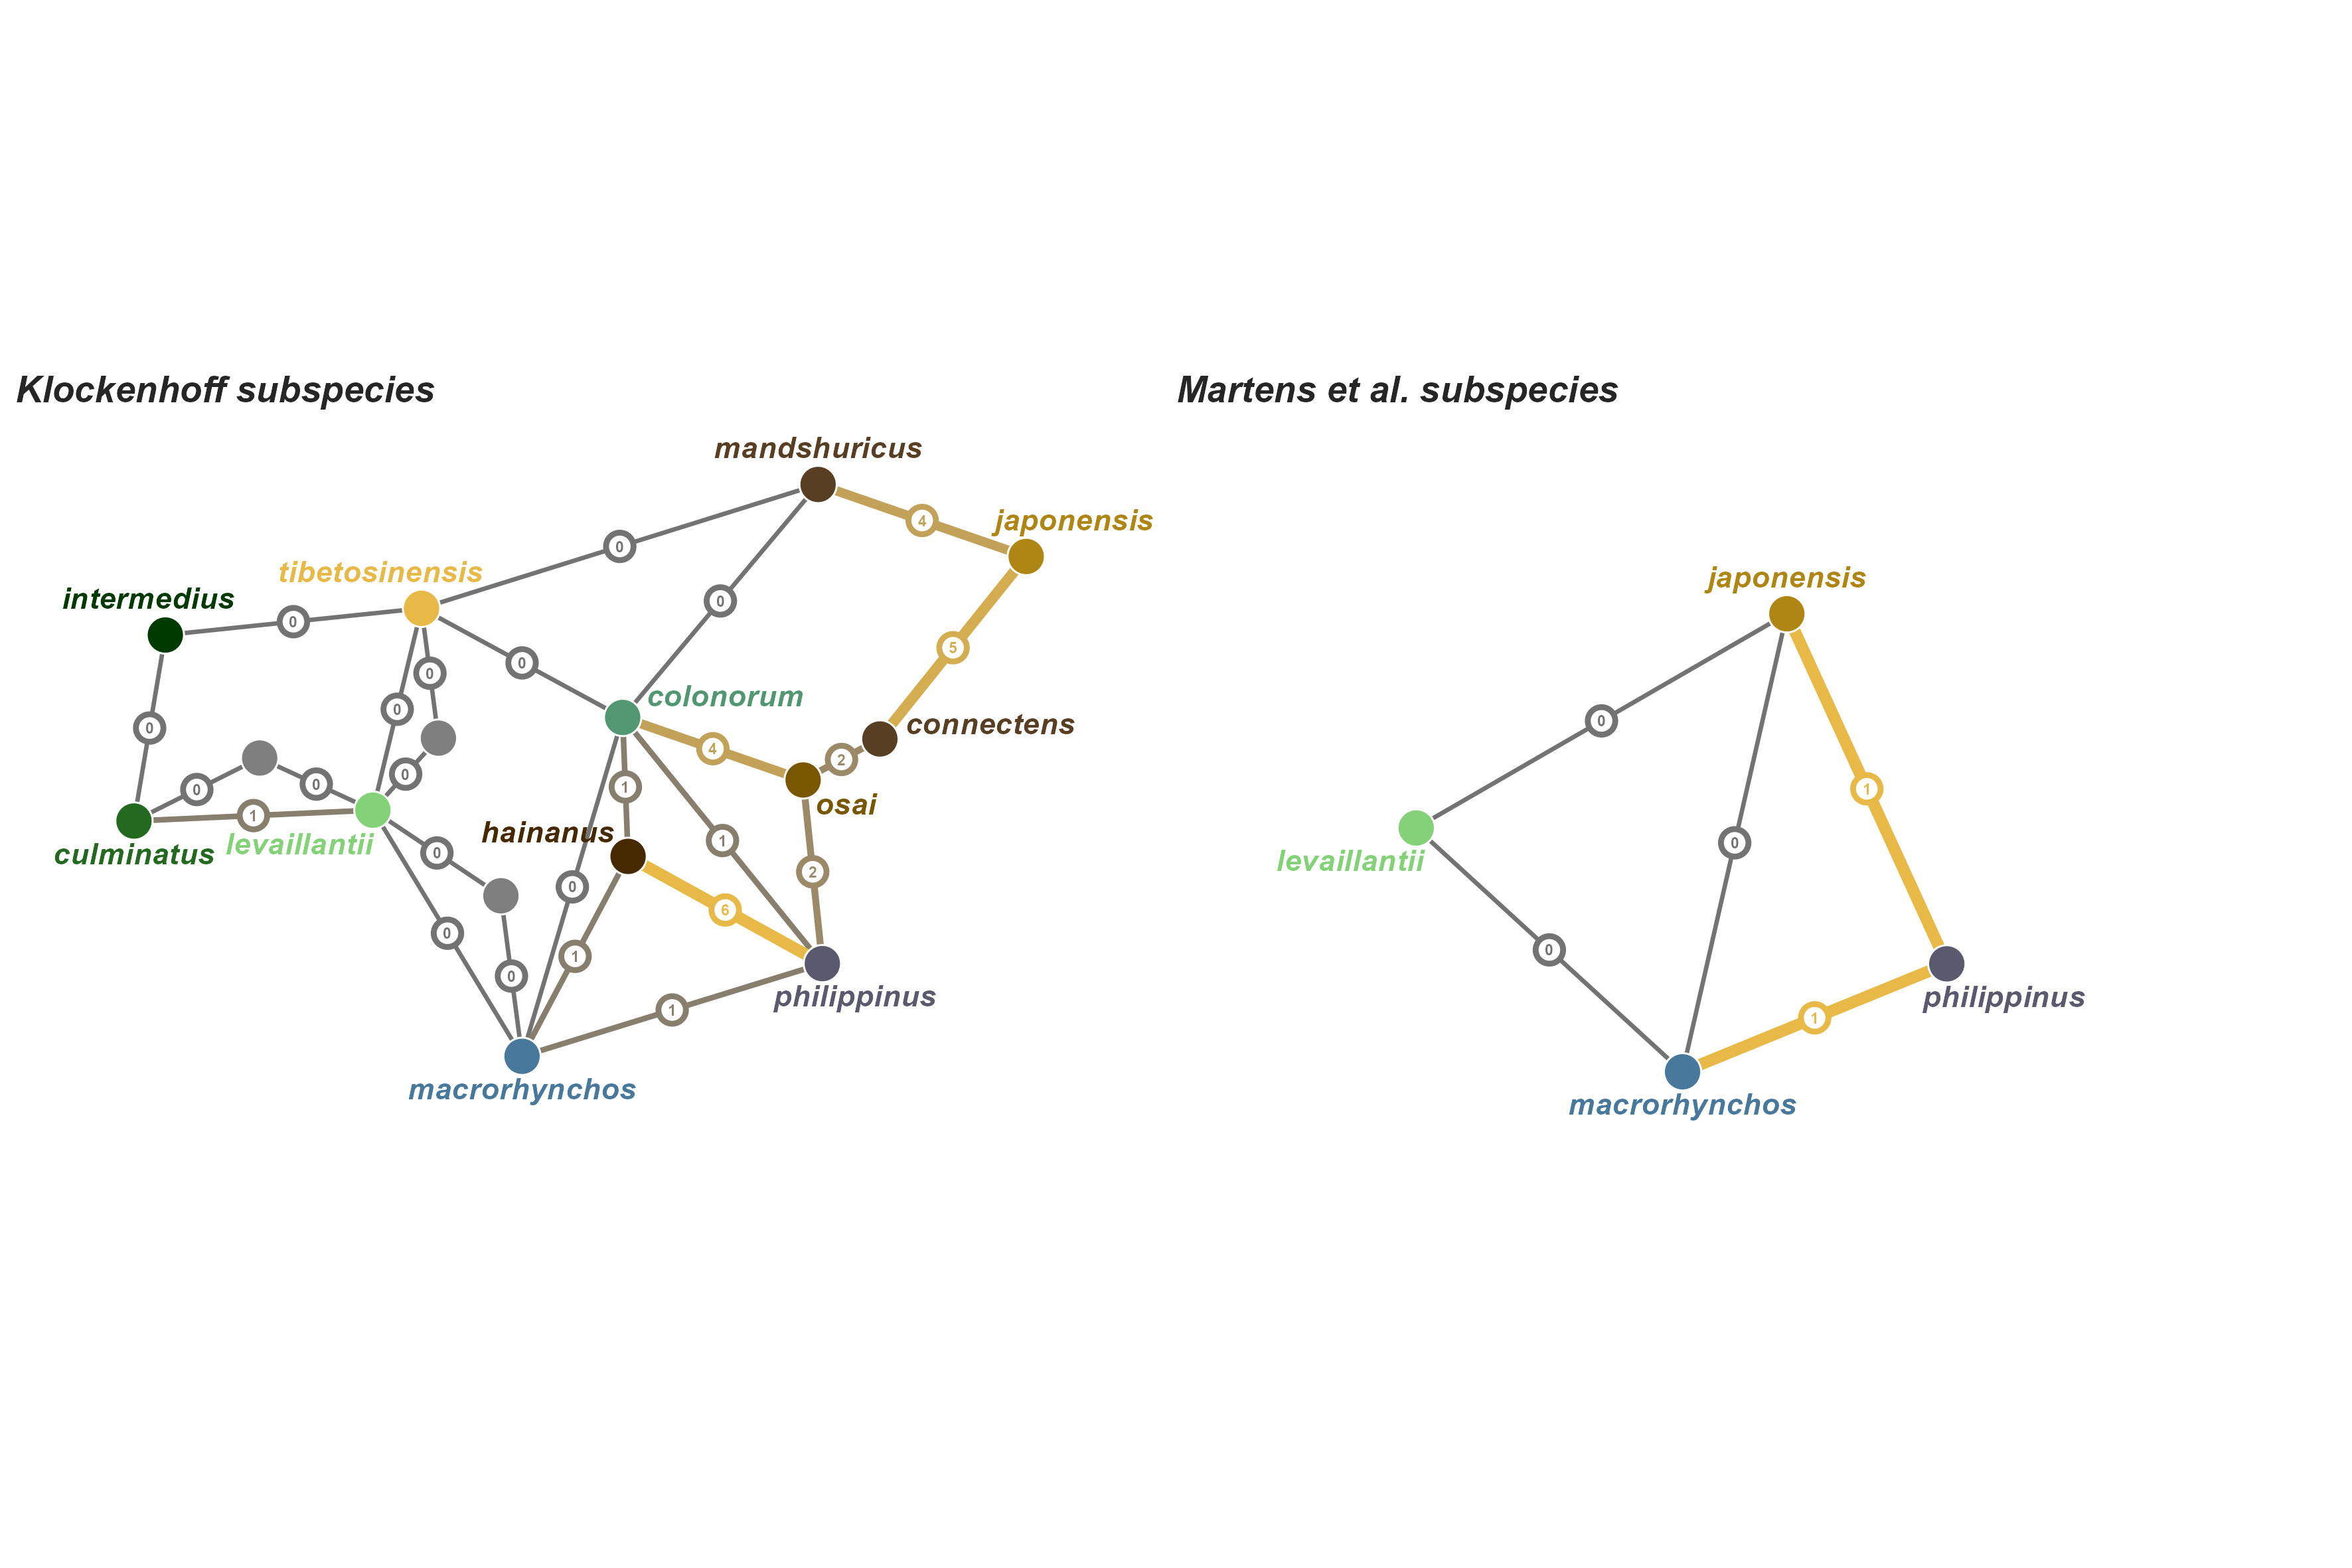
\includegraphics[width=0.9\linewidth]{../Figures/combined Subspecies Difference Plot} \caption{Number of measures (direct and composite) with significant differences between adjacent subspecies, using either Klockenhoff (1969) or Martens et al. (2000) subspecies boundaries. The number inside the line, along with line thickness and brightness, indicates a greater number of measures with an 85\% or higher chance of being different. Grey lines indicate that no measures between the two subspecies had >85\% chance of being different. Each subspecies is a different colour which corresponds to its map colour in Figure 2. Lines connect subspecies to their geographic neighbours. Gray dots on the Klockenhoff panel indicate hybrid zones.}\label{fig:countOfDifferencesPlot}
\end{figure}

\subsection{Assessing parasite-based subspecies proposal (Klockenhoff model)}\label{assessing-parasite-based-subspecies-proposal-klockenhoff-model}

Examination of contrasts from the pair-wise comparisons indicated that the majority of Klockenhoff's subspecies delineations based on feather parasites were not present in any one of our morphological measurements (Fig. \ref{fig:countOfDifferencesPlot}.
The contrasts revealed that the predicted distributions of many measures routinely overlapped with other proposed subspecies, including their neighbours (Fig. \ref{fig:klockContrasts}).
Such overlap would render identification of subspecies by physical markers difficult, and field identification nearly impossible.

There were several notable exceptions where a subspecies recognized by Klockenhoff stood out biometrically in our data set.
The strongest of these exceptions was \emph{C. m. japonensis}.
Compared to many other subspecies from Klockenhoff, \emph{C. m. japonensis} consistently showed larger bill measurements, particularly in Height at Nares and Exposed Culmen (Fig. \ref{fig:klockContrasts}).
For Height at Nares, the predicted distribution showed less than 1\% overlap with the predicted distribution of other subspecies (philippinus, culminatus, intermedius, osai, culminatus, intermedius), indicating near complete separation.
In these cases, the average median contrast (i.e., difference) was 5.8mm.
For Exposed Culmen, the subspecies philippinus, culminatus, intermedius, osai, culminatus, intermedius had less than 5\% overlap with the predicted distribution of \emph{C. m. japonensis}.
The average median contrast in this case is 9.92mm.
Other measures of \emph{C. m. japonensis} showed similar patterns, but less consistently and less dramatically.
Compared to its mainland neighbour \emph{mandshuricus}, height at nares (median contrast = 3.75mm, 95\% HDCI -1.78 to 9.35, 91.89\% probability of a no zero difference) and exposed culmen (6.84mm, 95\% HDCI -4.58 to 18.2, 88.98\%) also stand out as the most different.

Another exception is \emph{C. m. hainanus}.
Similar to \emph{C. m. japonensis}, height at nares stands out as lager than most other subspecies (average median contrast is 2.07mm).
In addition, measures of width at skin border and bill base length are also regularly larger than other subspecies (average median contrast for width at skin border 1.78mm; bill base length 3.46mm).
\emph{Corvus macrorhynchos japonensis} is the only subspecies to have any considerably larger measure than \emph{C. m. hainanus} (Height at nares).
However, compared to its near neighbour (\emph{C. m. colonorum}) it appears more similar than different.
Only bill base length is shows a sizeable non-overlap in distributions (3.7mm, 95\% HDCI -2.35 to 9.91, 89.84\%).

In contrast to the larger forms of \emph{japonensis} and \emph{hainanus}, \emph{intermidis} shows a pattern of smaller bill measurements, in particular width at nares (average median contrast: -4.12), and nares to bill tip (-1.52).
However, compared with its neighbours (\emph{culminatus} and \emph{tibetosinensis}) there are no discernible differences, with all distributions overlapping considerably.

Another subspecies that shows a pattern of smaller bill measurements is \emph{C. m. osai}.
It has considerably smaller measures of width at nares than 11 subspecies (3.31 mm), smaller measures of height at nares than 9 subspecies (3.43 mm), and smaller width at skin border than 8 subspecies (1.88 mm).
\emph{Corvus macrorhynchos osai} exists on a small island chain, neighbouring \emph{connectens} to its north east and \emph{colonorum} to its west.
It shows smaller measures in width (connectens: -2.29mm, 95\% HDCI -7.09 to 2.23, 13.09\%; colonorum: -2.93mm, 95\% HDCI -7.21 to 1.52, 8.06\%) and height at nares (connectens: -2.09mm, 95\% HDCI -6.13 to 2.06, 14.14\%; colonorum: -3.07mm, 95\% HDCI -7.17 to 1.29, 7.89\%), as well as width at skin border (connectens: -1.42mm, 95\% HDCI -4.25 to 1.69, 16.72\%; colonorum: -1.77mm, 95\% HDCI -4.22 to 0.69, 7.09\%) than both its nearest neighbours.

Outside of these two larger subspecies, and two smaller, all other proposed subspecies appeared to be statistically similar in most measures and not clearly separable as distinct subspecies on the basis of morphometrics.

\subsection{Assessing call-based subspecies proposal (Martens et al.~model)}\label{assessing-call-based-subspecies-proposal-martens-et-al.-model}

Compared to Klockenhoff, the comparisons between Martens' proposed subspecies reveal fewer differences (Fig. \ref{fig:martContrasts}).
Partly because there are dramatically fewer subspecies, but mainly because much of the variation occurs within the large subspecies divisions.
The only measure that appears to differ between subspecies is tarsus length, which is larger in \emph{C. m. macrorhynchos} compared to \emph{C. m. philippinus} (4.48mm, 95\% HDCI -3.64 to 12.55, 86.57\%; Fig. \ref{fig:martContrasts}).

\subsection{Exploration of measurements using inverse distance weighted maps}\label{exploration-of-measurements-using-inverse-distance-weighted-maps}

When treated as a single contiguous population, none of the morphometrics assessed singly showed a strong multi-modal distribution (see Fig. \ref{fig:overallPlot}), instead all revealed a unimodal normal distribution.

When morphometric variation was visualized in the IDW (Inverse Distance Weighted interpolation) maps, we hotspots of multiple measurements were revealed, in Height at Nares, Exposed Culmen, Tarsus Length, and Proximal Bill Surface Area that centred on Northern Japan, in particular Hokkaido; crows in this region included some of the largest measured specimens.
Not only did these crow specimens have the largest bills in absolute terms, but the ratio of Height at Nares to Tarsus Length as well as Proximal Bill Surface Area highlighted a tall bill even for their larger overall size (Fig. \ref{fig:idwMaps}).
This finding was reinforced by the difference in these measurements between Klockenhoff's definition of \emph{C. m. japonensis} and all other subspecies (Fig. \ref{fig:measuresMap}).

\begin{figure}
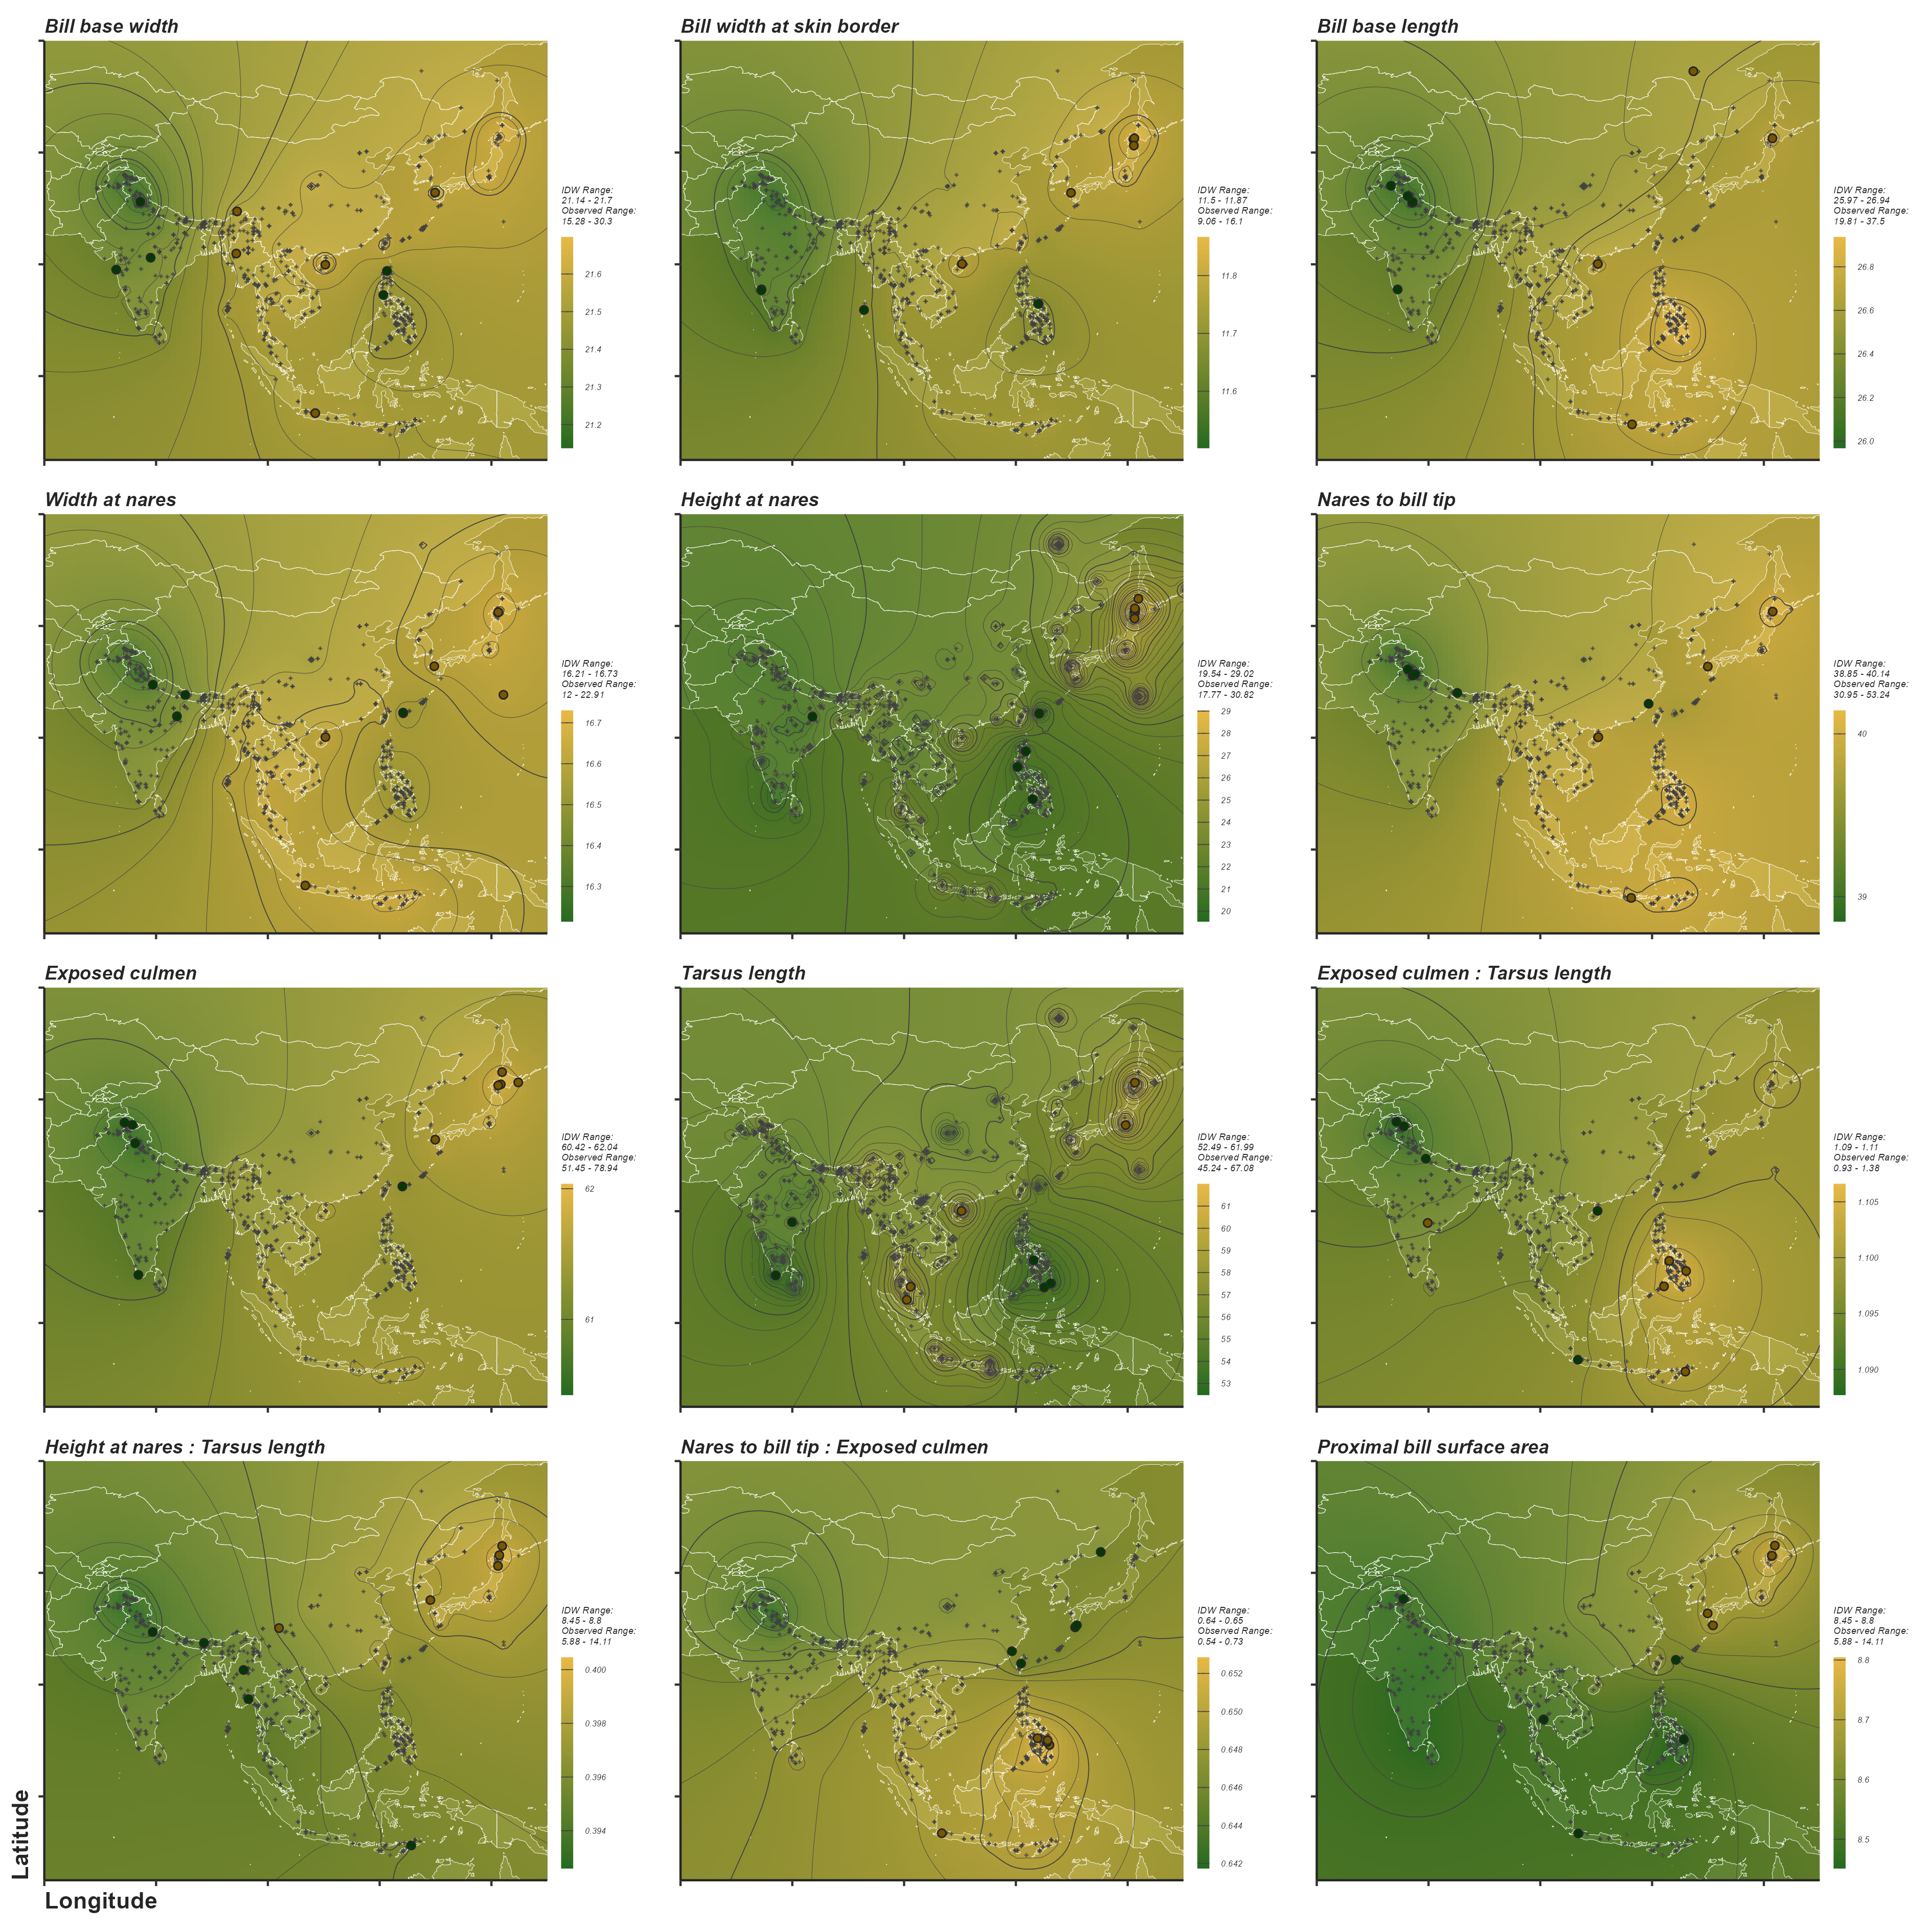
\includegraphics[width=0.9\linewidth]{../Figures/IDWmaps} \caption{Maps showing an interpolated inverse distance weighted heatmap of all collected measures and the four combined measures. Thicker contours match the line breakdowns shown on the legends to the right of the maps, three thinner contours exist between each break. For Nares to bill tip:Exposed Culmen, a higher number means the nares fall closer to the head, a lower number means the nares fall closer to the tip of the bill. Measures were scaled and colored with yellow at the high end of the scale and dark green at the lower end.}\label{fig:idwMaps}
\end{figure}

On the other end of the scale, the crows in northern India and Pakistan had some of the smallest bills in measures of width, length, and height.
They also had comparatively small tarsi compared to most crows outside of this area, suggesting an overall smaller bird.
However, the ratio of Height at Nares to Tarsus Length, as well as the ratio of Exposed Culmen to Tarsus Length, suggested that their bills were small even for their size.
Further emphasizing the small bill to body ratio in northern India and Pakistan was the lack of the same pattern in southern India.
In southern India crows had among the smallest tarsus measurements, but largely average bill measurements for their size.
The northern India and Pakistan crows also exhibited another unique characteristic: their nares were located further forward on their bills (a low Nares to Bill \url{Tip:Exposed} Culmen ratio) compared to \emph{C. macrorhynchos} from other areas.

Conversely, crows in the Philippines had nares that were placed further back on the bill, closer to the forehead.
The total Exposed Culmen in Philippine crows was largely average, but the Nares to Bill Tip measures were among the largest (\textgreater40 mm).
In addition, for their size (i.e., Tarsus Length) they tended to have long bills (i.e., Exposed Culmen) with the extra length tending to occur in the distal region of the bill (Nares to Bill Tip).
Width measures (Bill Base Width, Bill Width at Skin Border, and Width at Nares) did not show dramatic differences across the distribution, and largely followed overall patterns of Tarsus Length.
The separation of \emph{C. m. japonensis} by Klockenhoff seems to have the strongest support based on our measurements; this was reflected in the Bayesian comparisons (Fig. \ref{fig:klockContrasts}), as well as visible hotspots in the IDW maps (Fig. \ref{fig:idwMaps}).

Secondarily, the \emph{C. m. philippinus} subspecies (defined by both Klockenhoff and Martens et al.), while not showing major differences in the Bayesian comparisons, did appear to show some distinct characteristics in the IDW maps.

\subsection{Relationships of morphological measurements to climate factors}\label{relationships-of-morphological-measurements-to-climate-factors}

Our exploration of morphological measurements in relation to climatic measures showed several significant relationships between our measurements and mean annual temperature, temperature seasonality, or precipitation, although most explained less than 10\% of the variation in measurements (\emph{R\textsuperscript{2}} \textless{} 0.1; e.g., Fig. \ref{fig:climateComparisonMapTL}; Fig. \ref{fig:climateComparisonMapHN}).
There were two notable exceptions.

In the ratio Nares to Bill \url{Tip:Exposed} Culmen (Fig. \ref{fig:climateComparisonMapNtBTExCu}) we found a positive relationship between annual mean temperature and the Nares to Bill \url{Tip:Exposed} Culmen ratio (Gradient = 0.00092, R\^{}2 = 0.23, meaning as mean annual temperature increased, nares tended to fall more proximally on the bill, away from the tip.
There was also a significant, negative relationship between seasonality and Nares to Bill \url{Tip:Exposed} Culmen (Gradient = -3.2e-05), meaning in areas with more temperature variability throughout the year, nares tended to fall farther forward, towards the tip of the bill.

\begin{figure}
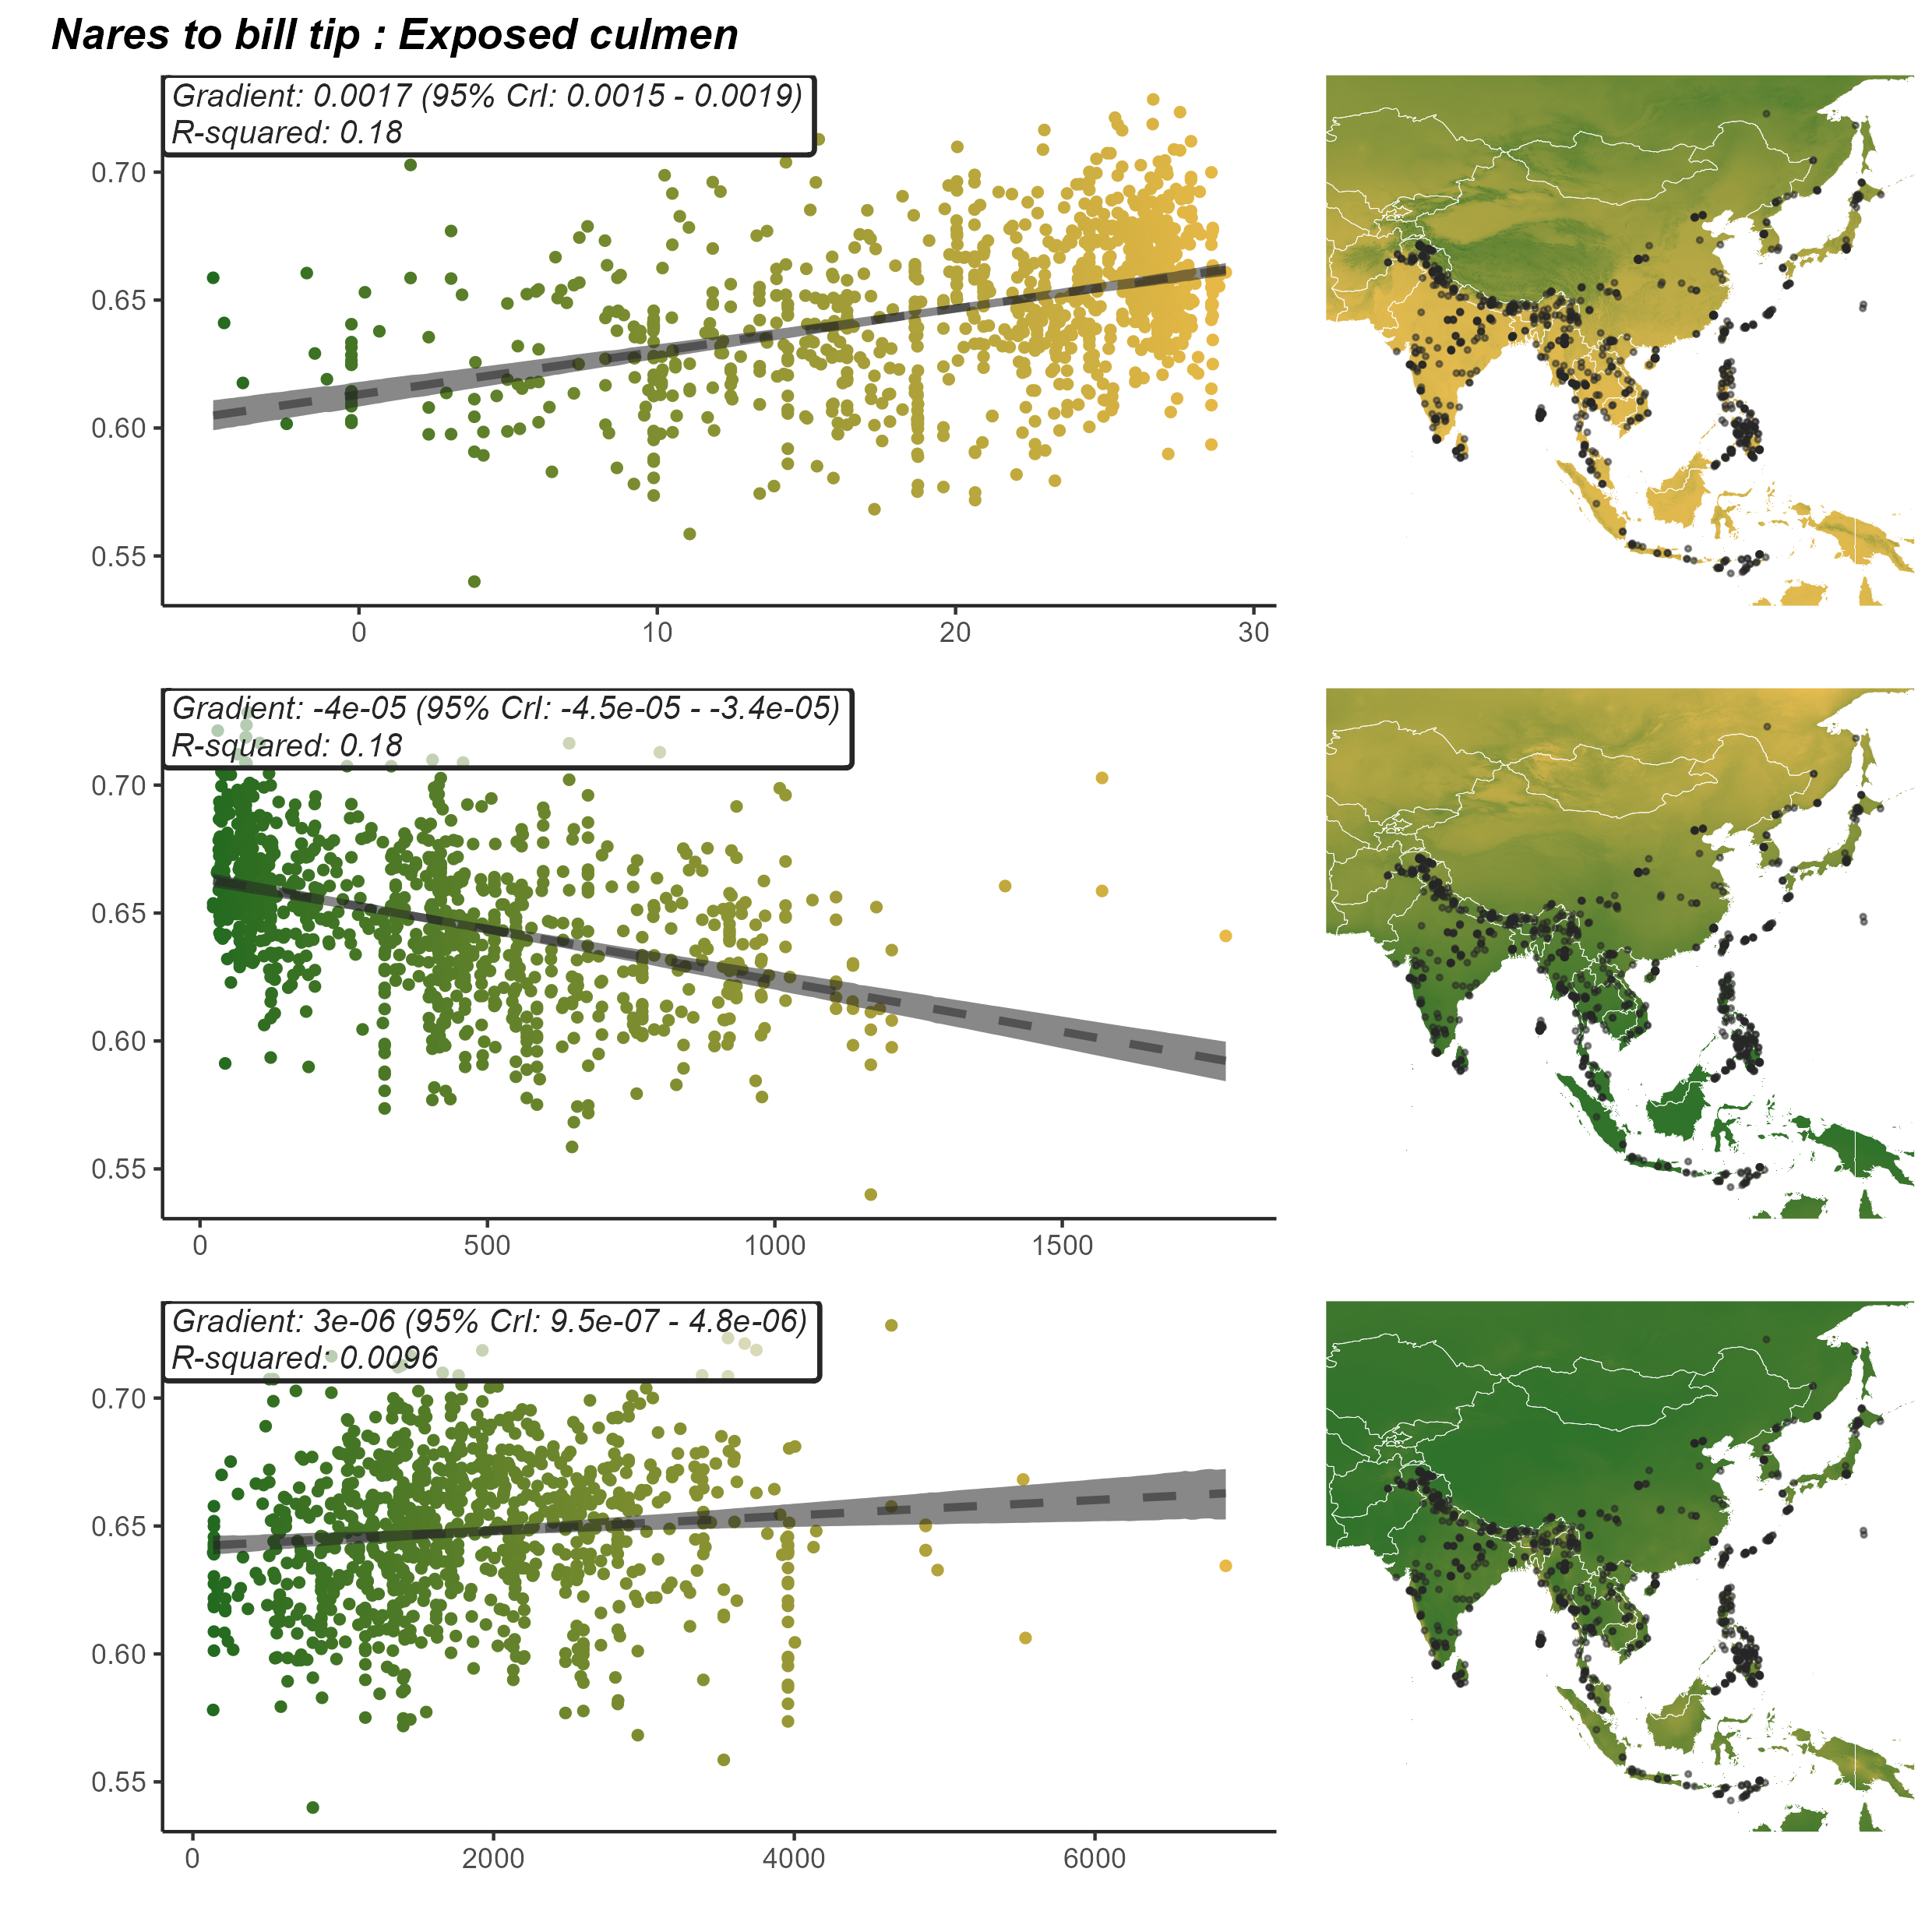
\includegraphics[width=0.9\linewidth]{../Figures/climMap_NtBT.ExCu} \caption{Measures of the ratio of Nares to Bill Tip : Exposed Culmen in relation to annual mean temperature, temperature seasonality, and annual precipitation. Lower values are represented by dark green and higher values are represented by yellow.}\label{fig:climateComparisonMapNtBTExCu}
\end{figure}

In our measure of Proximal Bill Surface Area (Fig. \ref{fig:climateComparisonMapPBSA}) we found a negative relationship between annual mean temperature and Proximal Bill Surface Area relative to body size (Gradient = -0.028, R\^{}2 = 0.19, meaning in areas with a higher annual mean temperature, crow bills tended to have a smaller surface area near the face.
We also found a positive relationship between Proximal Bill Surface Area and temperature seasonality (Gradient = 0.0014) meaning in areas with higher seasonality, proximal bill surface area tended to be larger.

\begin{figure}
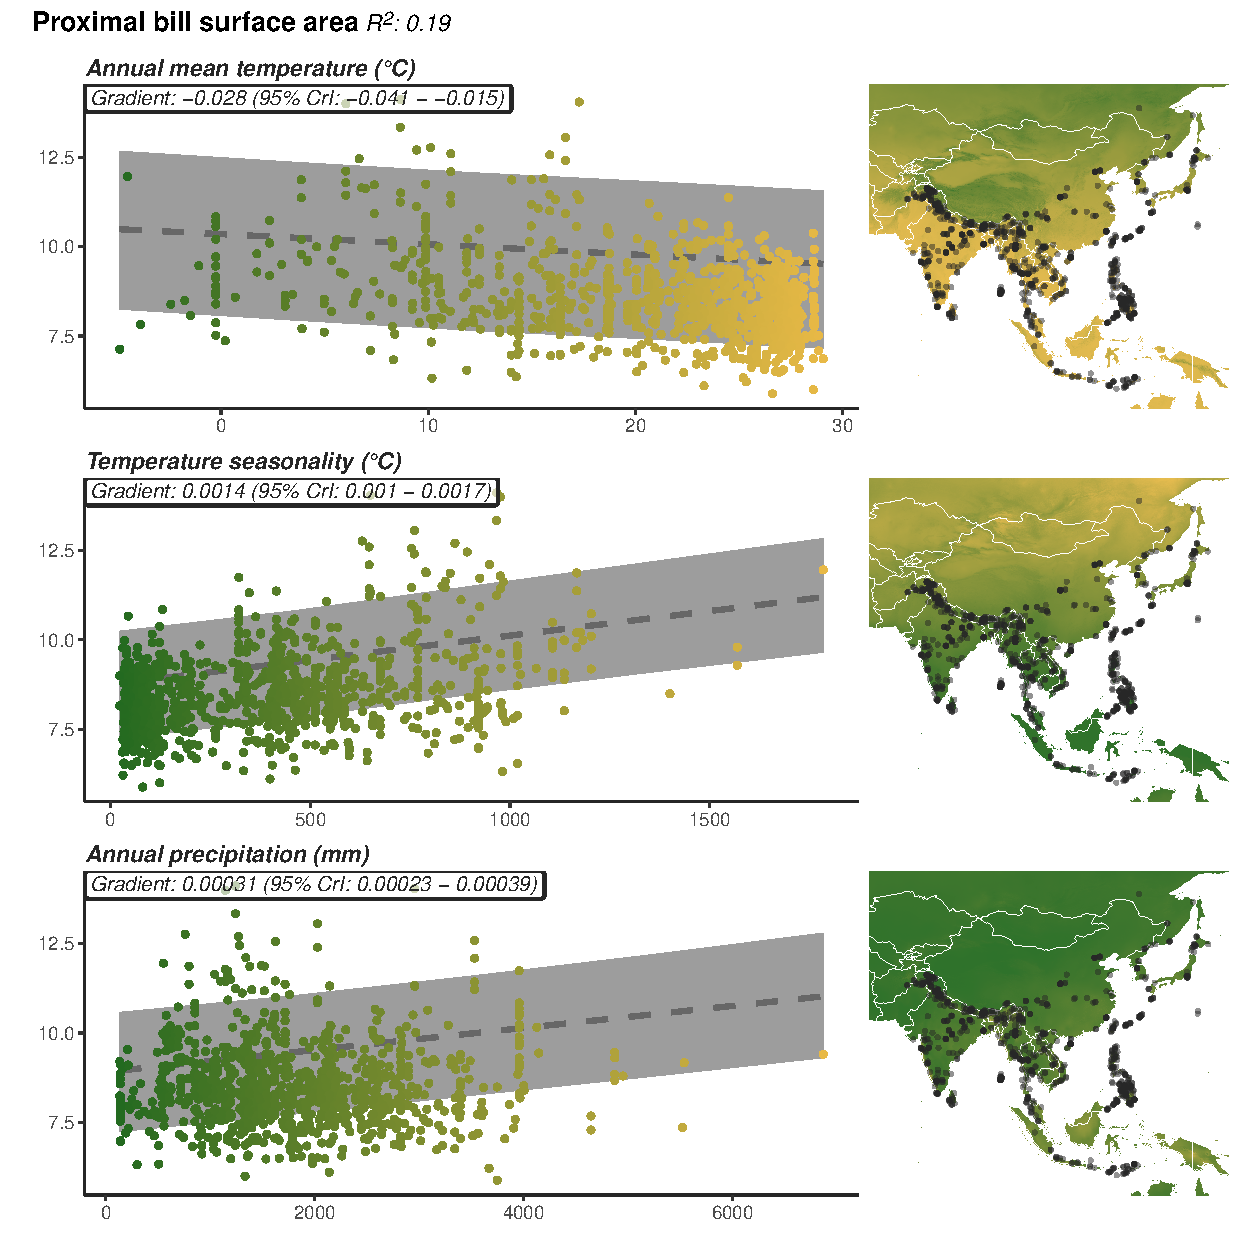
\includegraphics[width=0.9\linewidth]{../Figures/climMap_ExCuNtBTxHaNaTaLe} \caption{Measures of the ratio of Nares to Bill Tip : Exposed Culmen in relation to annual mean temperature, temperature seasonality, and annual precipitation. Lower values are represented by dark green and higher values are represented by yellow.}\label{fig:climateComparisonMapPBSA}
\end{figure}

\section{Discussion}\label{discussion}

To characterize the geographic variation in Jungle Crow (\emph{Corvus macrorhynchos}) morphology, and to test existing subspecies propositions, we measured key morphological characteristics from over 1000 museum specimens.
Bayesian comparisons of differences revealed no evidence for overall sexual dimorphism, nor any sexual dimorphism within any proposed subspecies.

The biogeography of subspecies proposed by Klockenhoff (\citeproc{ref-klockenhoff_zur_1969}{1969}), and Martens (\citeproc{ref-martens_calls_2000}{2000}) were also largely not reflected in our measures of morphology, with several notable exceptions: \emph{Corvus m. japonensis} as defined by Klockenhoff exhibited larger bills even for their body size than other subspecies, as did \emph{C. m. hainanus}.
Whereas both \emph{C. m. intermedius} and \emph{C. m. osai} showed smaller bills than expected for their body size.
We found very few clear differences in morphology between the Martens et al.~groups, with the exception of shorter tarsi (i.e., smaller size) in \emph{C. m. philippinus}.

We also explored the appearance of areas of phenotypic interest, outside of the previous definitions of subspecies.
Our explorations revealed Japan, the Philippines, and northern India and Pakistan had the most distinct phenotypes.
The Japanese crows appeared larger overall and had disproportionately taller bills.
The northern Indian and Pakistani crows appeared smaller overall and had disproportionately smaller bills with nares positioned closer to the bill tip.
The Philippine crows also appeared smaller overall and had disproportionately longer bills with nares positioned closer to the forehead.
Outside of these hotspots, the remainder of the distribution appeared gradated and morphological differences appeared relatively minor.

Factors we could not account for such as age {[}beyond limiting the sample to adult crows; Jones et al. (\citeproc{ref-jones_age-related_2002}{2002}); Reid et al. (\citeproc{ref-reid_impact_2024}{2024}){]}, health, diet (\citeproc{ref-acquarone_effects_2002}{Acquarone et al., 2002}; \citeproc{ref-pierce_diet_2004}{Pierce \& McWilliams, 2004}; \citeproc{ref-heiss_growth_2009}{Heiss, Clark \& McGowan, 2009}), and differing maturation rates between sexes may have influenced crow size (\citeproc{ref-badyaev_growing_2002}{Badyaev, 2002}), and the degree of sex dimorphism in our samples (although we detected marginal sex differences within the proposed subspecies).
Therefore, a study aiming to fully examine sex differences within \emph{C. macrorhynchos} would do well to control for these factors.
However, the low level of sexual dimorphism in our sample, with males being marginally larger on average, is not particularly unexpected as previous descriptions of this species have indicated males and females are indistinguishable in the field (\citeproc{ref-whistler_popular_2008}{Whistler, 2008}).
This is also a common pattern seen in other \emph{Corvus spp.} {[}e.g., \emph{C. splendens}, \emph{C. corone}, \emph{C. frugilegus}; Madge (\citeproc{ref-billerman_large-billed_2020}{2020}){]}.
Previous studies have suggested lower size dimorphism reflects a lack of intra-sexual competition common in monogamous species, as well as smaller inter-sexual differences in parental care (\citeproc{ref-owens_sexual_1998}{Owens \& Hartley, 1998}).
This taken together with field guide descriptions and personal behavioural observations {[}Pers. Obs.; Alamshah (\citeproc{ref-alamshah2024morphological}{2024}){]} suggests that \emph{C. macrorhynchos} is a socially monogamous species, where both parents care for the young, potentially relieving the pressures seen in competitive communal nesting species (\citeproc{ref-babbitt_selection_2007}{Babbitt \& Frederick, 2007}).

While the lack of dimorphism appeared to align with previous assertions regarding \emph{C. macrorhynchos}, the geographic patterns in morphology did not.
The majority of subspecies suggested by Klockenhoff did not appear clearly in our data.
For example, crows on either side of the boundary between \emph{culminatus} and \emph{intermedius} were similar in all measures.
In addition, Klockenhoff suggested four distinct subspecies in southeast Asia, where neither the Bayesian comparison nor IDW maps of our data revealed any clear evidence of morphometric boundaries in this region.
Klockenhoff's boundaries were based on the differences in feather parasites.
These parasites may have been subject to different environmental pressures or limited in their ability to travel between hosts (\citeproc{ref-diblasi_phoretic_2018}{DiBlasi et al., 2018}; \citeproc{ref-sweet_role_2018}{Sweet \& Johnson, 2018}).
This could render a disconnect or varying relationship between the physical characteristics of the crows and the species make-up of these parasites at different scales (\citeproc{ref-dube_microclimate_2018}{Dube et al., 2018}; \citeproc{ref-bodawatta_ecological_2022}{Bodawatta et al., 2022}).
Martens et al.'s subspecies had a large east to west distribution, particularly their \emph{C. m. japonensis} designation which covers Japan to Afghanistan and encompassed both the largest and smallest crows that we measured.
Therefore, comparing morphometric measures between their \emph{japonensis} and any other subspecies resulted in a near complete overlap.
Martens et al.'s splits were based on call structure, with field data conducted in only three locations.
As such, they may have missed key boundaries existing with their larger definitions.
For example, we highlighted the distinctly larger crows of Japan and smaller crows of the Philippines, while Martens et al.~did not sample any of the island populations.
A fuller comparison of the morphometrics to call structure would require more extensive sampling of crow calls across \emph{C. macrorhynchos}' distribution.

The larger size of tarsus and bill of \emph{C. macrorhynchos} in Japan may have several different explanations.
Our largest measures were centred around Hokkaido, which is near the northernmost edge of the crows' distribution.
These crows were not only larger in most measures but also had taller bills in relation to their bodies.
A tall bill could be a result of sexual selection (see \citeproc{ref-babbitt_selection_2007}{Babbitt \& Frederick, 2007} for an example sexual selection driven differences), but this seems unlikely, because male and female measurements were very similar.
Bergmann's rule suggests that the crows might be bigger here to deal with the colder temperatures, and a taller bill might also provide a physiological advantage, perhaps warming inspired air in this environment (\citeproc{ref-geist_nasal_2000}{Geist, 2000}).
Additionally, the other resident \emph{Corvus spp.} (\emph{Corvus corone}) in Japan appears to be larger than their European counterparts (\citeproc{ref-madge_crows_1999}{Madge \& Burn, 1999}; \citeproc{ref-tobias_avonet_2022}{Tobias et al., 2022}).
When plotting Height at Nares against climatic measures, we found a significant but weak negative relationship between Height at Nares and mean annual temperature (Fig. \ref{fig:climateComparisonMapHN}).
This may be due to the overall smaller measurements of crows in the Himalayas, which included the lowest mean annual temperatures.
We found a stronger positive relationship between Height at Nares and temperature seasonality which suggests temperature variability might have more of an impact on bill height than the annual average temperature.
Tarsus Length followed a similar, albeit weaker, pattern to bill height, with a weak negative relationship between Tarsus Length and annual mean temperature and a slightly stronger positive relationship between Tarsus Length and seasonality (Fig. \ref{fig:climateComparisonMapTL}).
This suggests that overall body size might be marginally affected by temperature and seasonality, but it is likely not a major driver.

Another morphological pattern to consider is the placement of the nares.
The strongest relationship found was the negative relationship between the Nares to Bill Tip : Exposed Culmen ratio and annual mean temperature (Fig. \ref{fig:climateComparisonMapNtBTExCu}).
This showed that in areas with higher annual mean temperatures, nares tended to fall closer to the base of the bill, while in areas with lower mean annual temperatures, the nares tended to fall closer to the tip.
We also found a positive relationship between temperature seasonality and Nares to Bill Tip : Exposed Culmen ratio, meaning that higher seasonal temperature variability correlated with nares being closer to the tip of the bill.
It is possible that this may be an adaptation for cold climates, where a longer nasal passage would allow air temperature to be regulated in the bill before reaching the body (\citeproc{ref-geist_nasal_2000}{Geist, 2000}).

It is important to note that these measures of morphology do not encompass all aspects of \emph{C. macrorhynchos}' phenotypic variation, and more evidence is needed to identify areas of divergence or subspecies delineations.
There are examples of cryptic species belonging to a diversity of taxa widely distributed across Asia (\citeproc{ref-olsson_non-monophyletic_2005}{Olsson et al., 2005}; \citeproc{ref-outlaw_pliocene_2008}{Outlaw \& Voelker, 2008}; \citeproc{ref-burton_geographical_2010}{Burton \& Nietsch, 2010}; \citeproc{ref-shankar_king_2021}{Shankar et al., 2021}; \citeproc{ref-dufresnes_speciation_2025}{Dufresnes et al., 2025}), and evidence that cryptic species are just as likely to appear in Eurasian birds (\citeproc{ref-pfenninger_cryptic_2007}{Pfenninger \& Schwenk, 2007}).
Cryptic species are known to be important in properly describing biodiversity (\citeproc{ref-voda_cryptic_2015}{Vodă et al., 2015}); as such, further investigation using genetic methods could be justified.
The results of our exploration highlight areas such as the Philippines, the Himalayas, and Northern Japan, that would potentially be prime candidates for targeted investigation via genetic sampling, vocal analysis, or additional morphometrics.
Future studies should focus on these morphological ``hotspots'' as potential areas of heightened divergence.

\section{Acknowledgements}\label{acknowledgements}

\subsection{Data and code availability}\label{data-and-code-availability}

For all analysis we used R (v.4.4.2) (\citeproc{ref-base}{R Core Team, 2024}), and R Studio (v.2024.12.0+467) (\citeproc{ref-rstudio}{Posit team, 2024}). For general data manipulation we used glue (v.1.8.0) (\citeproc{ref-glue}{Hester \& Bryan, 2024}), and tidyverse (v.2.0.0) (\citeproc{ref-tidyverse}{Wickham et al., 2019}). For project and code management we used here (v.1.0.1) (\citeproc{ref-here}{Müller, 2020}), tarchetypes (v.0.11.0) (\citeproc{ref-tarchetypes}{Landau, 2021a}), and targets (v.1.9.0) (\citeproc{ref-targets}{Landau, 2021b}). For visualisation we used the following as expansions from the tidyverse suite of packages: ggdist (v.3.3.2) (\citeproc{ref-ggdist2024a}{Kay, 2024a},\citeproc{ref-ggdist2024b}{b}), and patchwork (v.1.3.0) (\citeproc{ref-patchwork}{Pedersen, 2024}). Other packages we used were brms (v.2.22.0) (\citeproc{ref-brms2017}{Bürkner, 2017b}, \citeproc{ref-brms2018}{2018b}, \citeproc{ref-brms2021}{2021b}), crew (v.0.10.2) (\citeproc{ref-crew}{Landau, 2024}), ggpubr (v.0.6.0) (\citeproc{ref-ggpubr}{Kassambara, 2023}), knitr (v.1.49) (\citeproc{ref-knitr2014}{Xie, 2014}, \citeproc{ref-knitr2015}{2015}, \citeproc{ref-knitr2024}{2024}), Metrics (v.0.1.4) (\citeproc{ref-Metrics}{Hamner \& Frasco, 2018}), tidybayes (v.3.0.7) (\citeproc{ref-tidybayes}{Kay, 2024c}), and tidyselect (v.1.2.1) (\citeproc{ref-tidyselect}{Henry \& Wickham, 2024}). To generate typeset outputs we used bookdown (v.0.42) (\citeproc{ref-bookdown2016}{Xie, 2016}, \citeproc{ref-bookdown2025}{2025}), and rmarkdown (v.2.29) (\citeproc{ref-rmarkdown2018}{Xie, Allaire \& Grolemund, 2018}; \citeproc{ref-rmarkdown2020}{Xie, Dervieux \& Riederer, 2020}; \citeproc{ref-rmarkdown2024}{Allaire et al., 2024}). To manipulate and manage spatial data we used , and terra (v.1.8.29) (\citeproc{ref-terra}{Hijmans, 2025}). To run models and explore model outputs we used , and performance (v.0.12.4) (\citeproc{ref-performance}{Lüdecke et al., 2021}).

\subsection{Author contributions}\label{author-contributions}

We thank Dr.~Anne Clark for the immense amount of financial, logistical, and intellectual support she provided throughout the collection of this data, without which this would not have been possible.
We also thank Dr.~Kevin McGowan, not only for access to the museum at the Cornell Lab of Ornithology but also for his advice and support throughout development and implementation of this project.
We thank the following museum curators for graciously allowing access to their collections and providing their expertise and logistical support: Augie Kramer at the American Museum of Natural History, Ben Marks at the Field Museum of Natural History, Christopher Milensky at the Smithsonian National Museum of Natural History, and Hein van Grouw at the Natural History Museum at Tring.

\subsection{Competing interests}\label{competing-interests}

The authors declare that they have no known competing financial interests or personal relationships that could have appeared to influence the work reported in this paper.

\subsection{Funding}\label{funding}

This research did not receive any specific grant from funding agencies in the public, commercial, or not-for-profit sectors.

\clearpage

\section{Supplementary material}\label{supplementary-material}

\begin{figure}
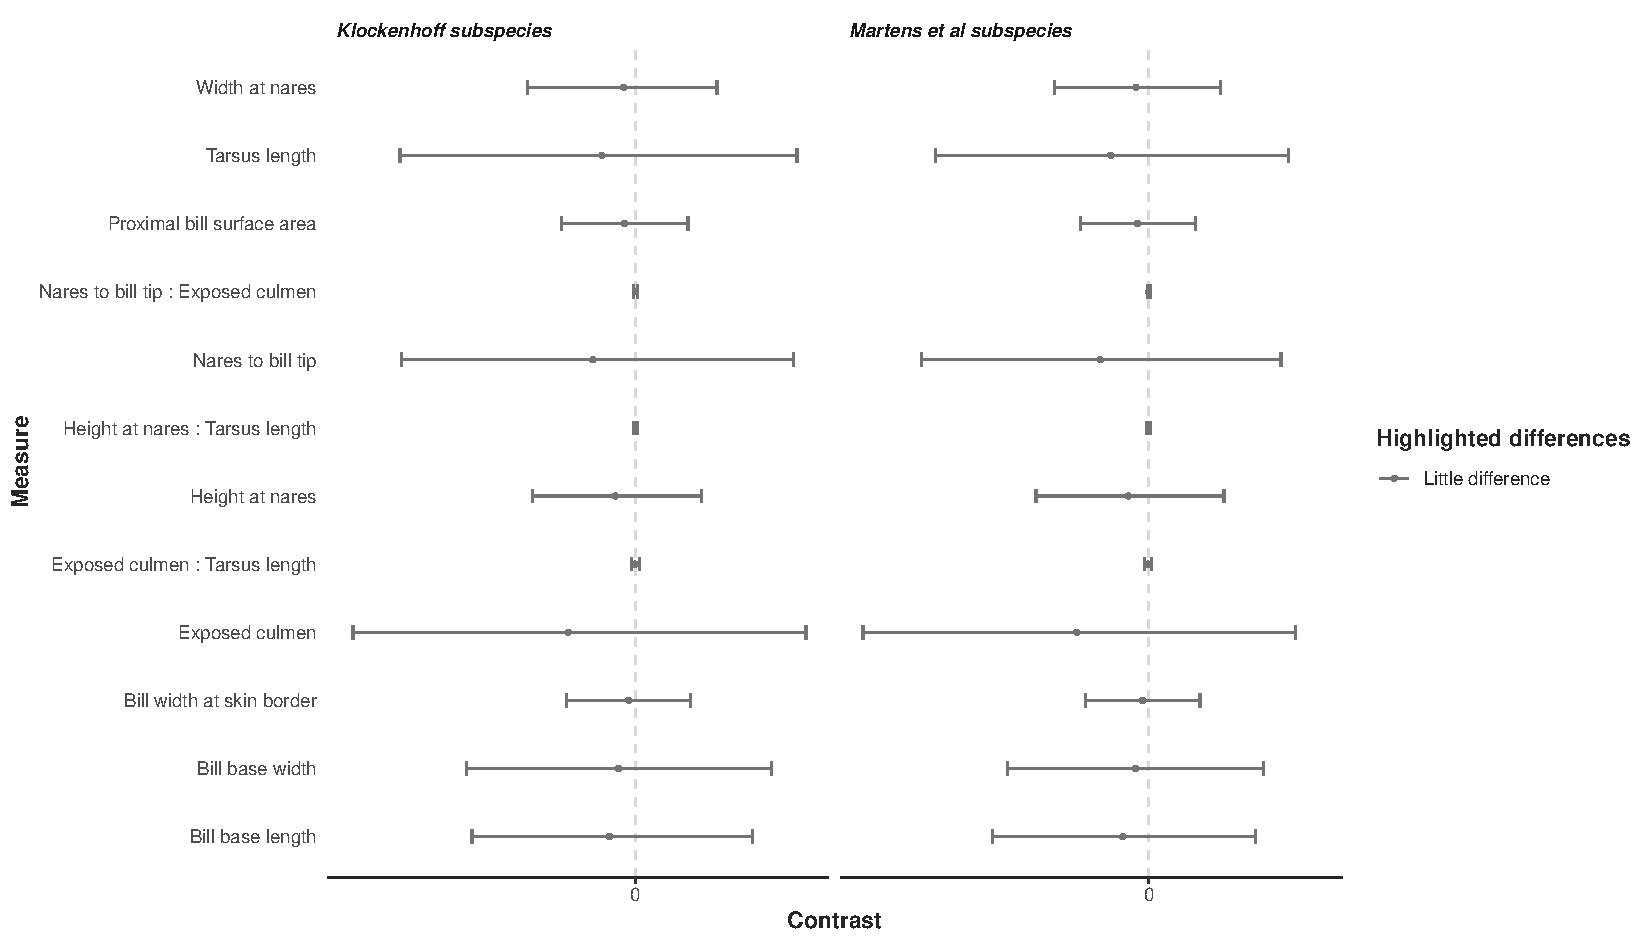
\includegraphics[width=0.9\linewidth]{../Figures/_HDCI_sex_contrasts} \caption{The contrasts' distributions illustrating the difference between male and female crows. The lines indicate the 95\% Highest Density Credible Interval surroundding the median.}\label{fig:sexContrasts}
\end{figure}

\begin{figure}
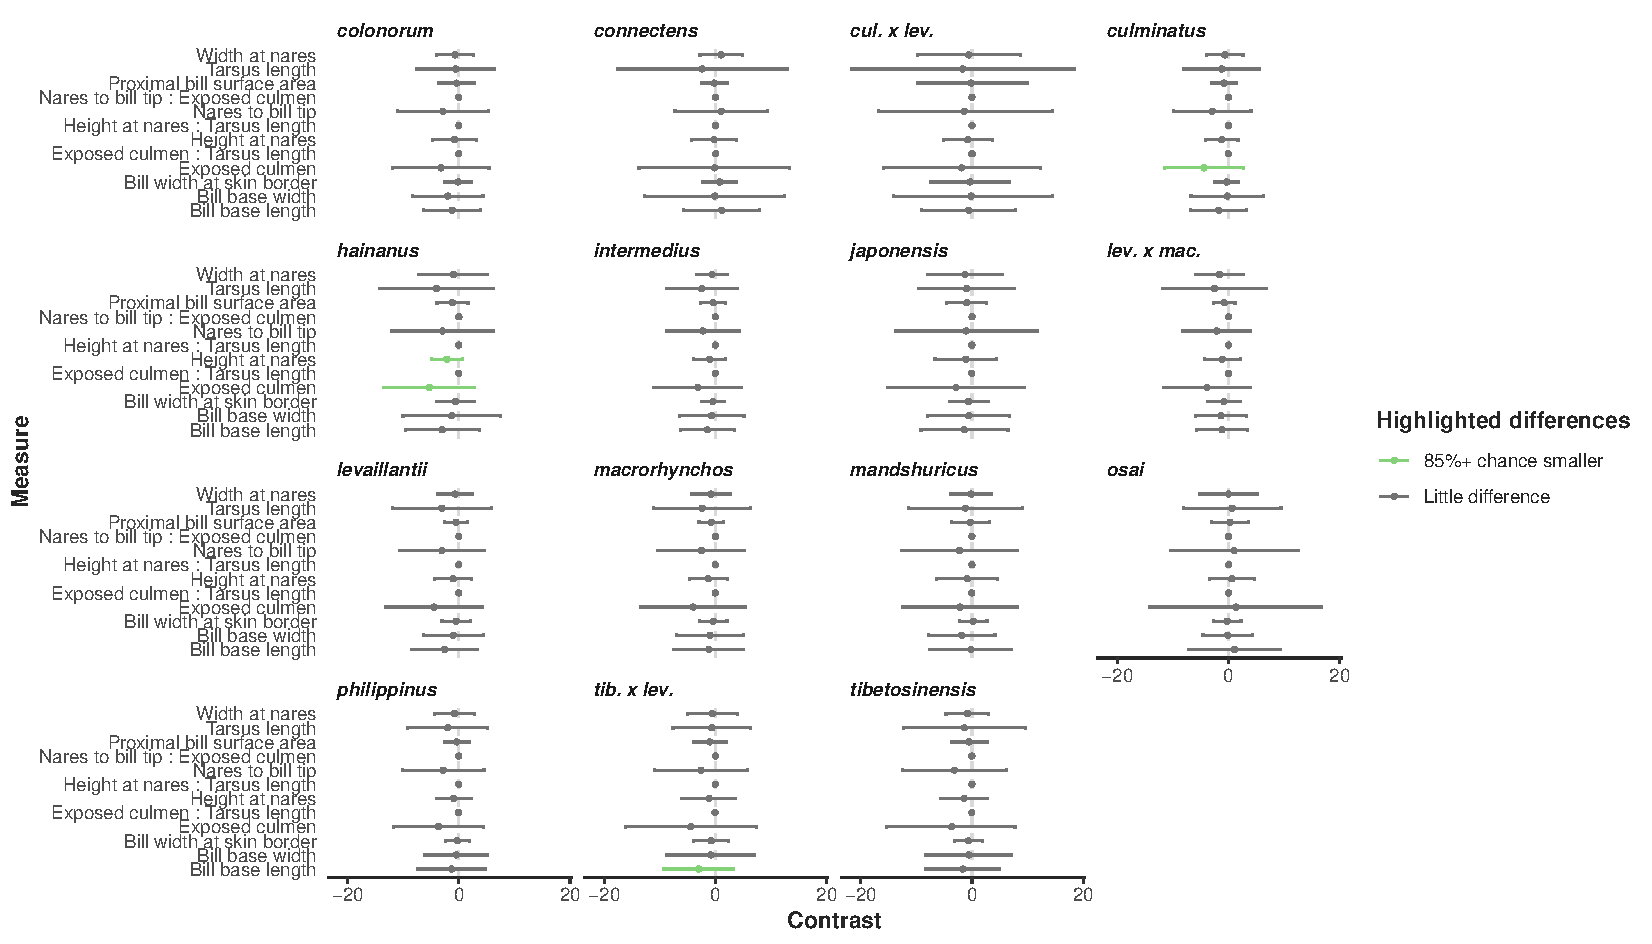
\includegraphics[width=0.9\linewidth]{../Figures/klockSpecies_HDCI_intraSubspeciesSex_contrasts} \caption{The contrasts' distributions illustrating the difference between male and female crows. The lines indicate the 95\% Highest Density Credible Interval surroundding the median.}\label{fig:sexKlockContrasts}
\end{figure}

\begin{figure}
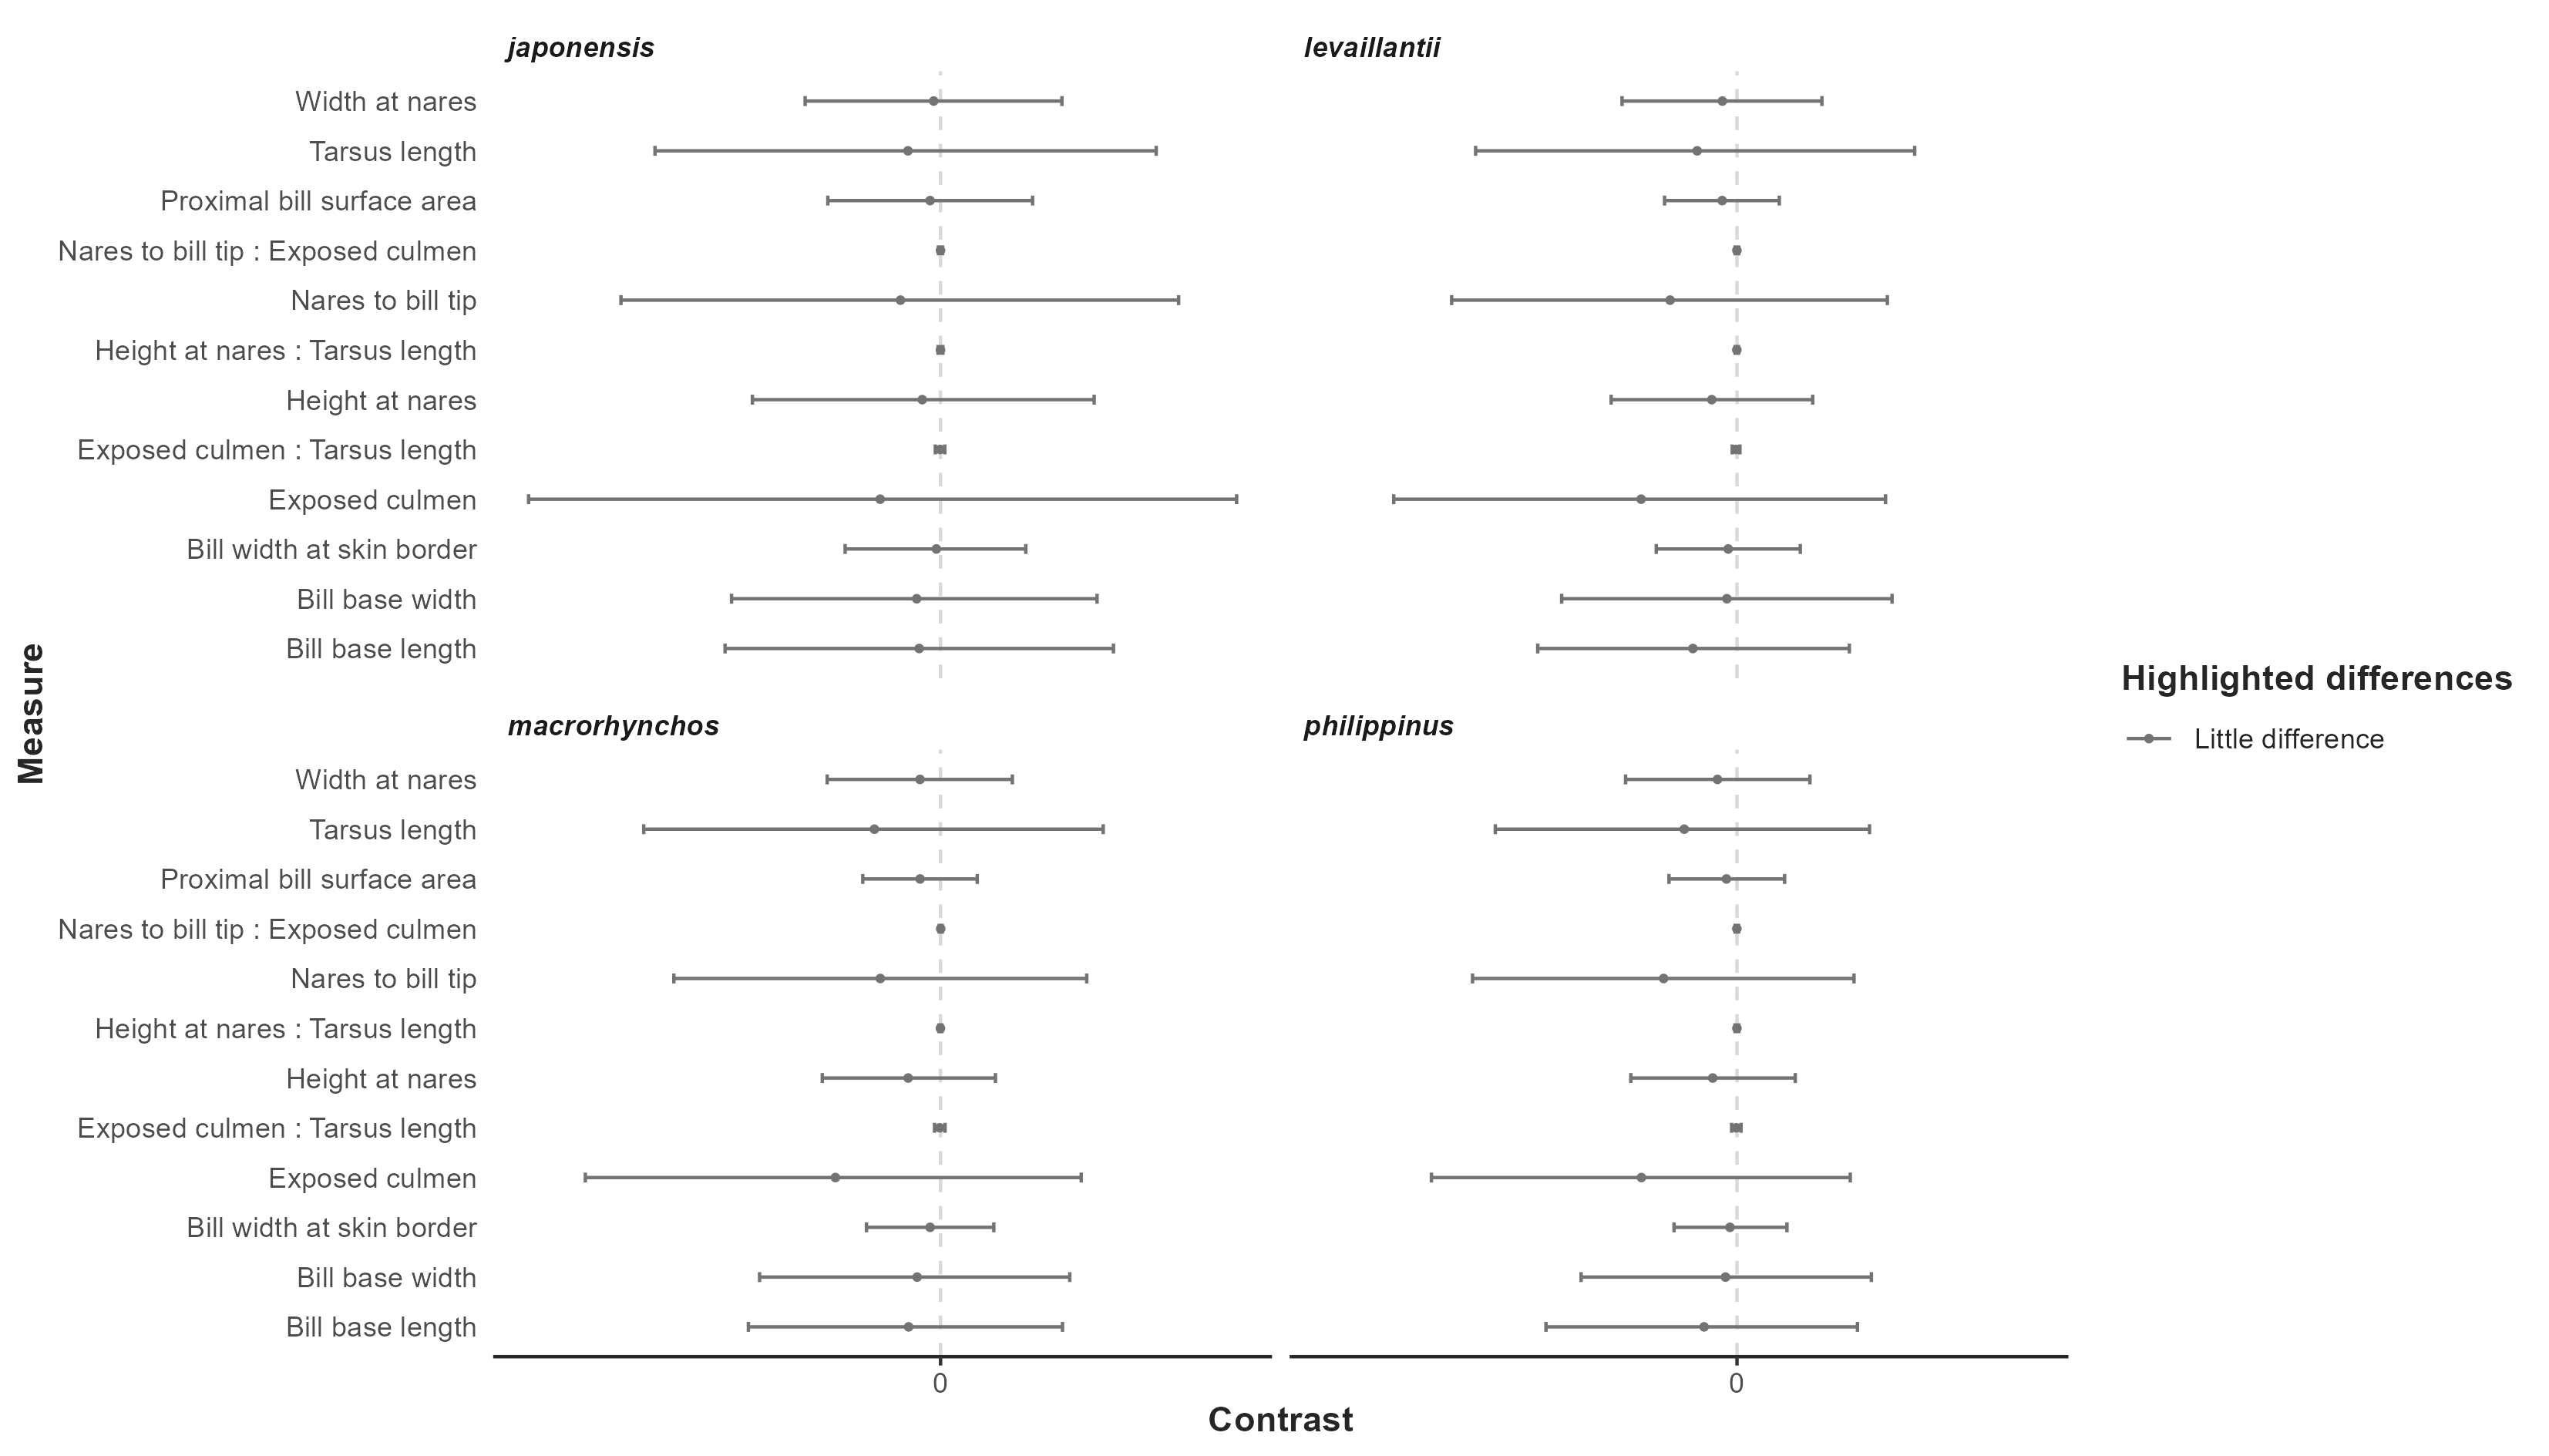
\includegraphics[width=0.9\linewidth]{../Figures/martSpecies_HDCI_intraSubspeciesSex_contrasts} \caption{The contrasts' distributions illustrating the difference between male and female crows. The lines indicate the 95\% Highest Density Credible Interval surroundding the median.}\label{fig:sexMartensContrasts}
\end{figure}

\begin{figure}
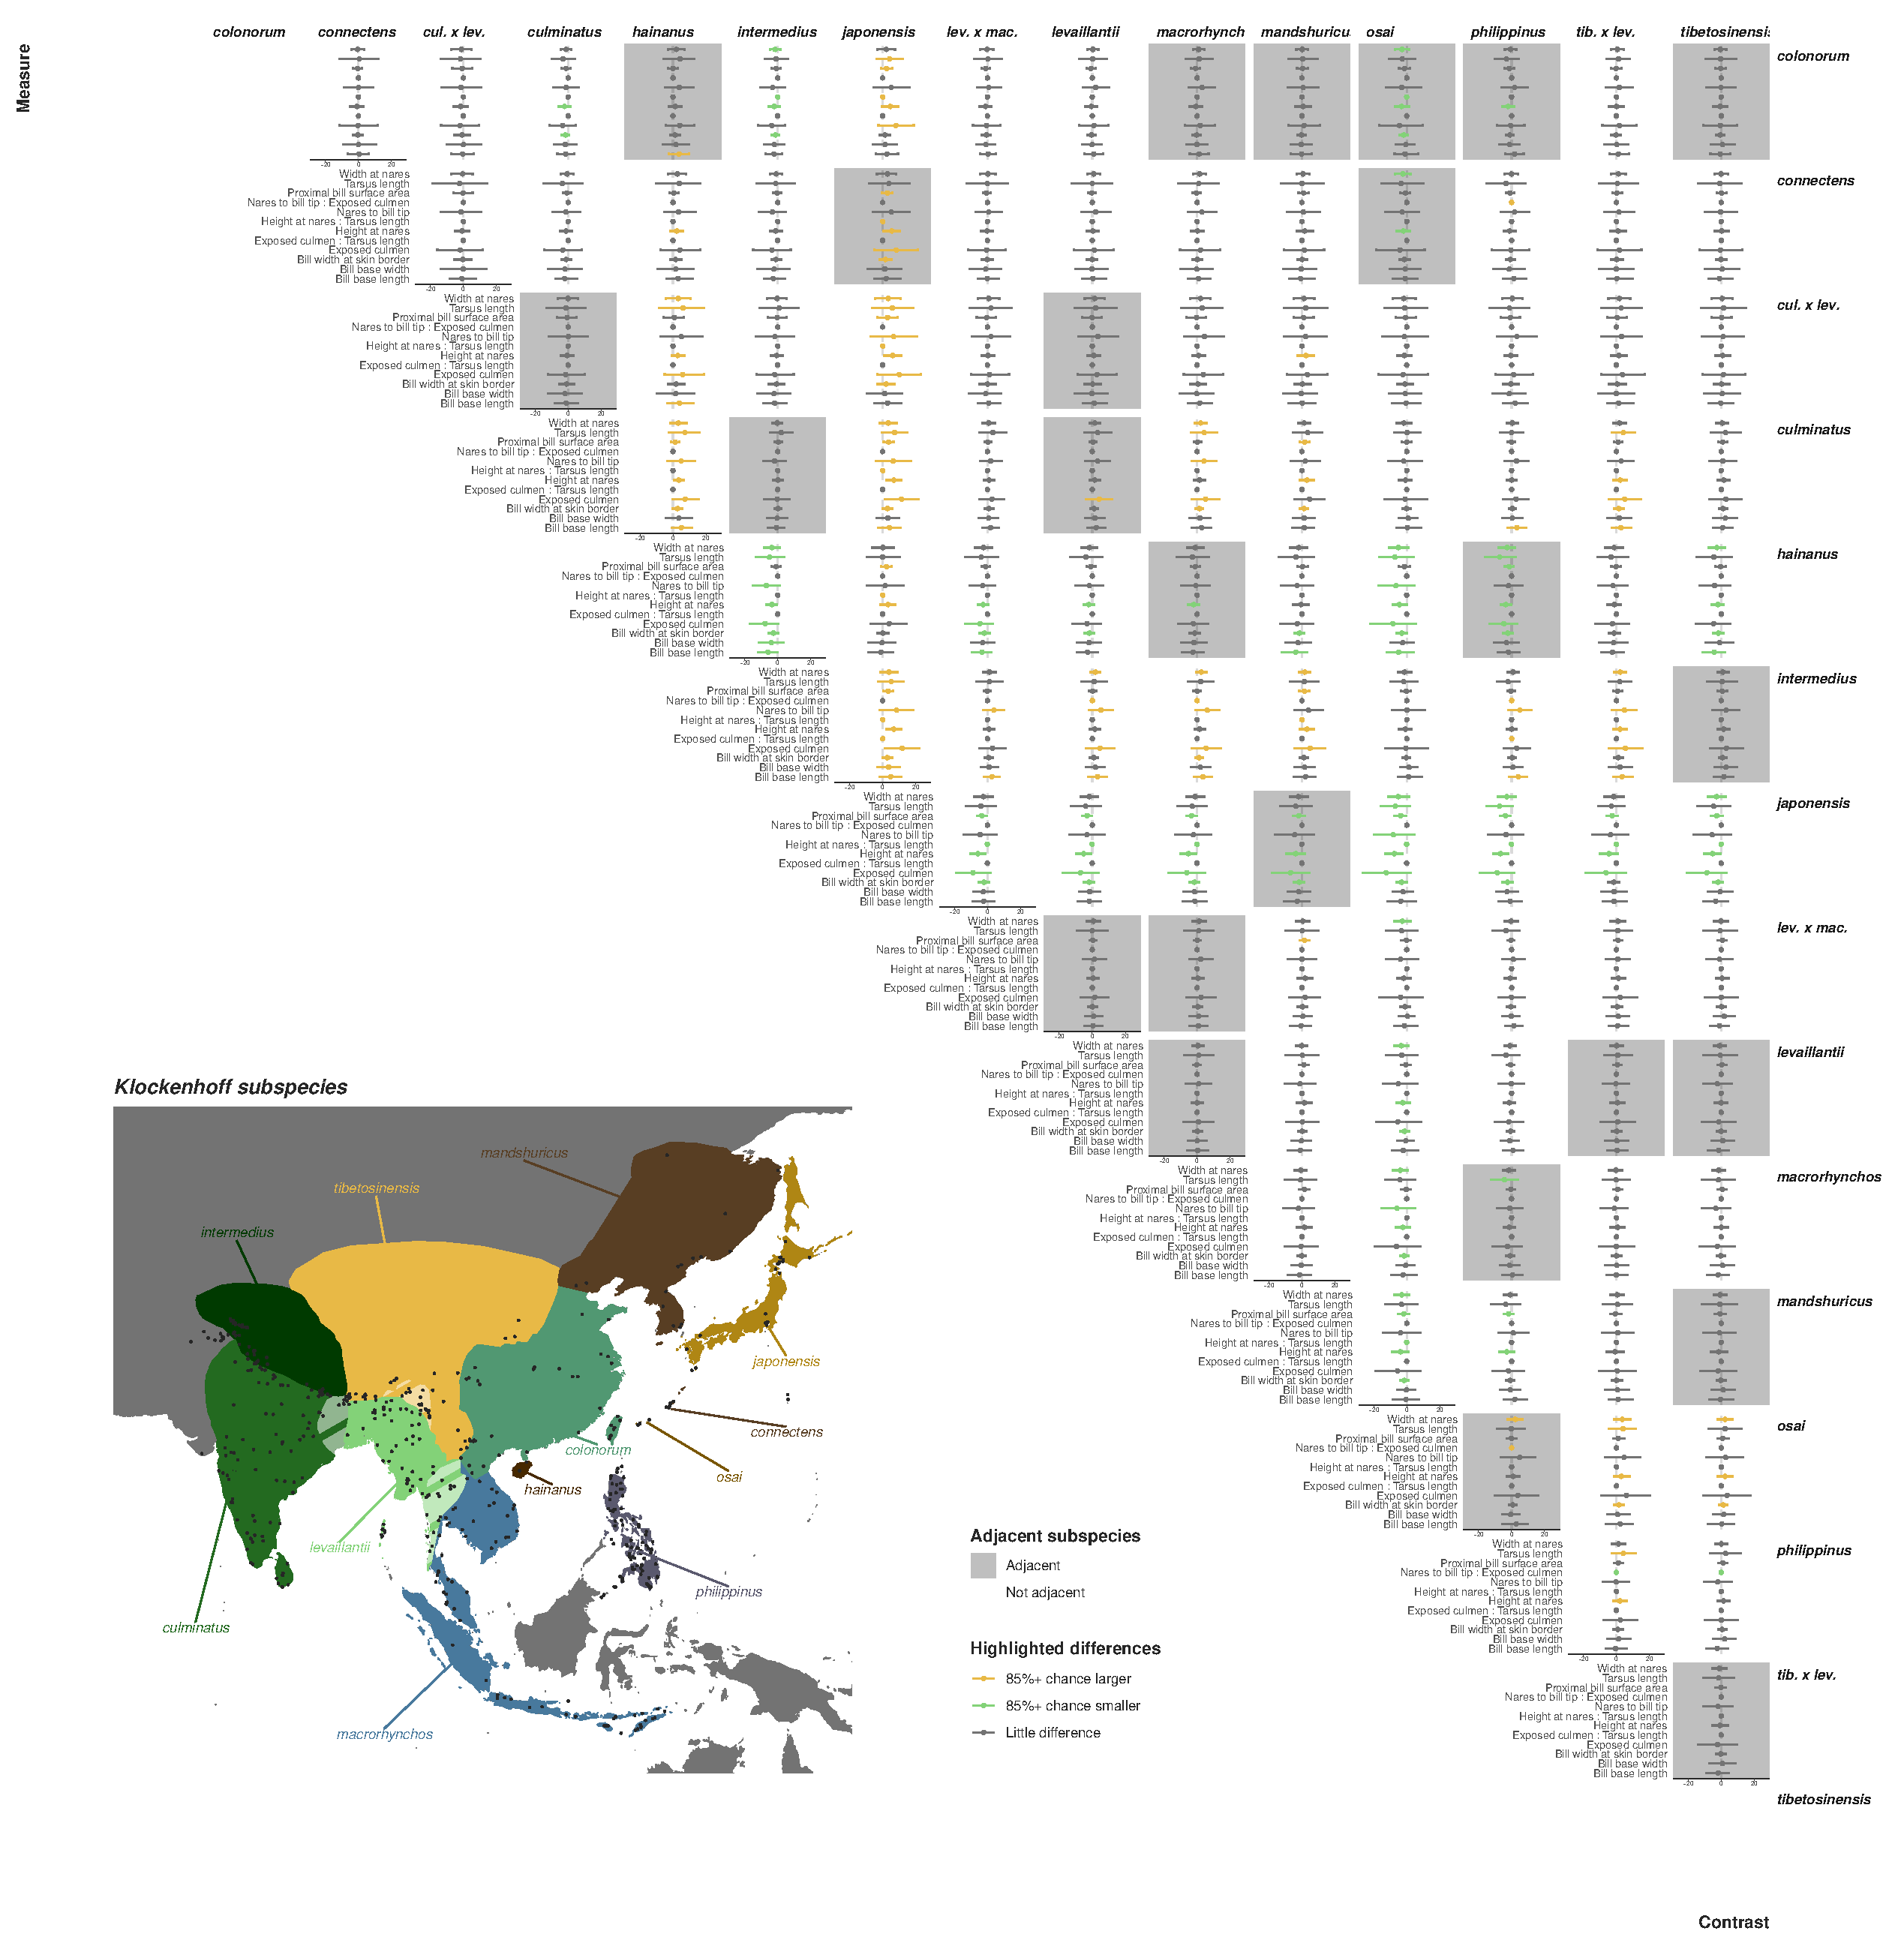
\includegraphics[width=0.9\linewidth]{../Figures/klockSpecies_HDCI_contrasts} \caption{The contrasts' distributions illustrating the difference between all Klockenhoff proposed subspecies. The lines indicate the 95\% Highest Density Credible Interval surrouinding the median.}\label{fig:klockContrasts}
\end{figure}

\begin{figure}
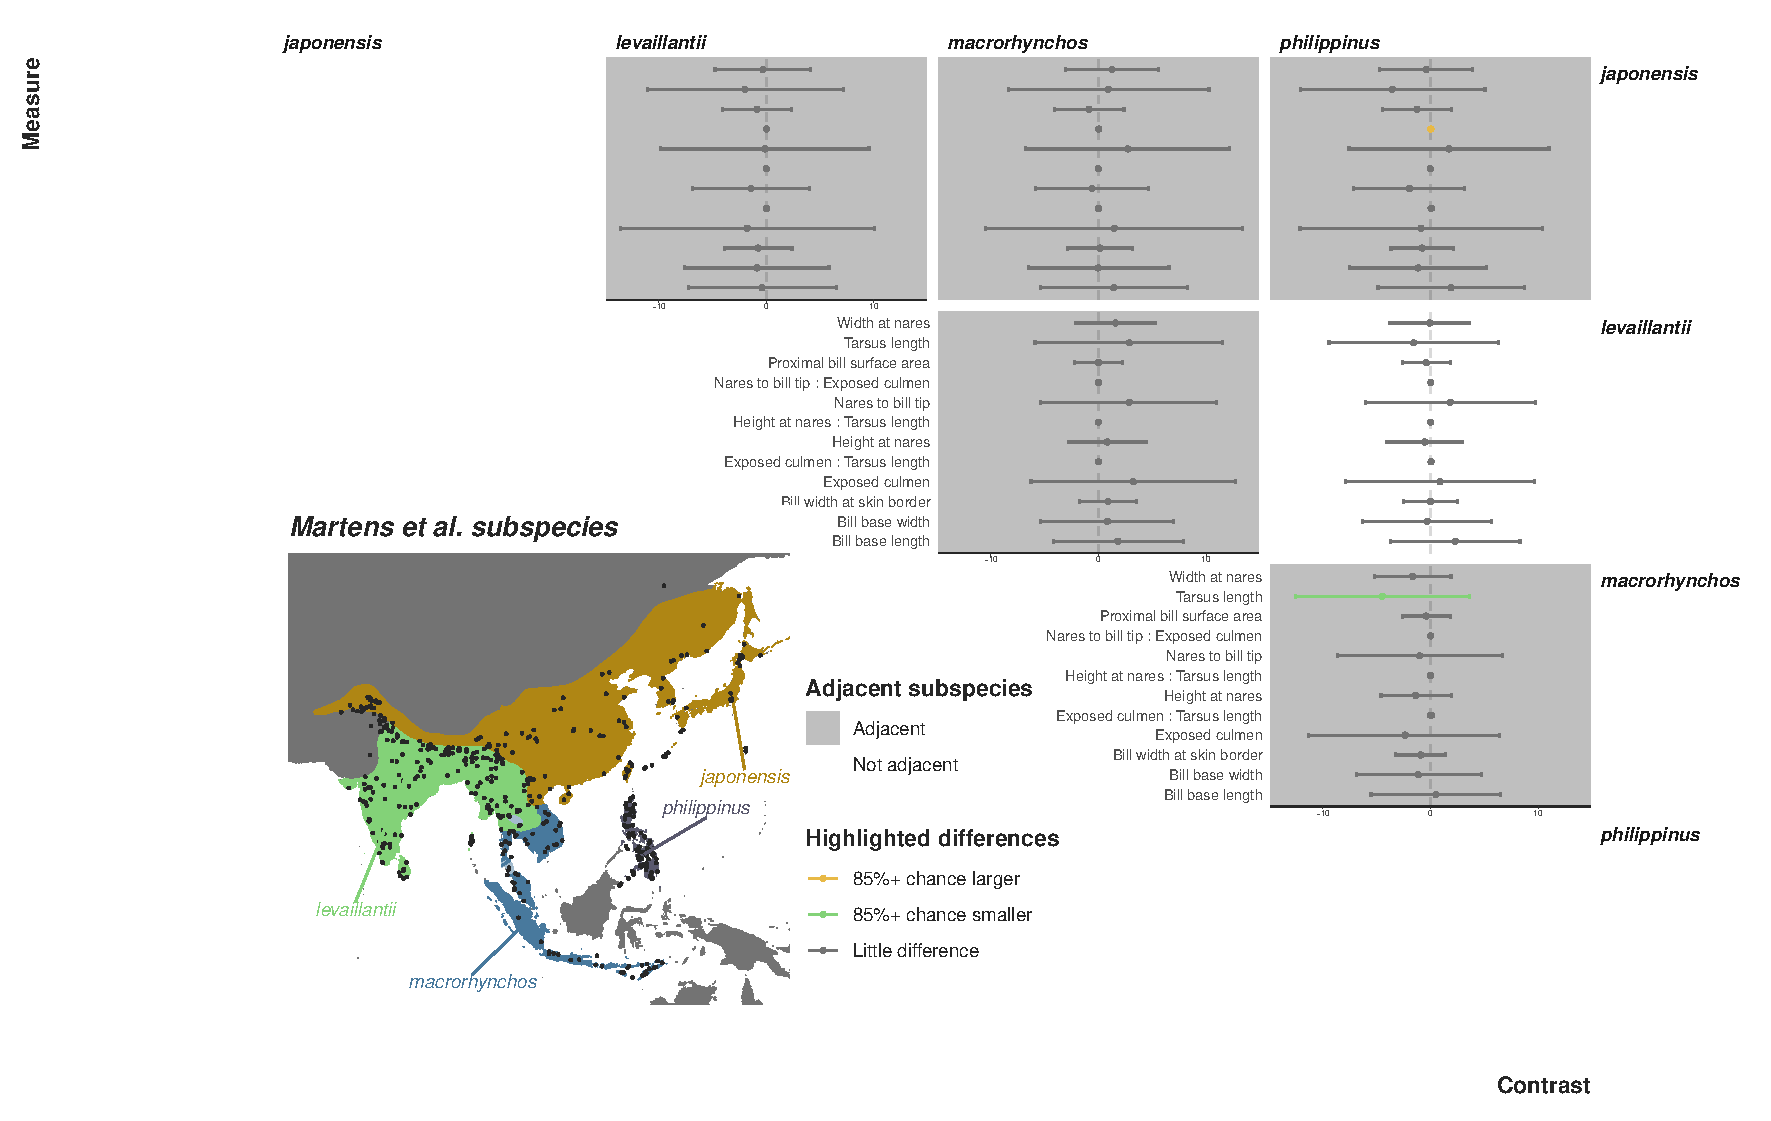
\includegraphics[width=0.9\linewidth]{../Figures/martSpecies_HDCI_contrasts} \caption{The contrasts' distributions illustrating the difference between all Martens proposed subspecies. The lines indicate the 95\% Highest Density Credible Interval surrouinding the median.}\label{fig:martContrasts}
\end{figure}

\begin{figure}
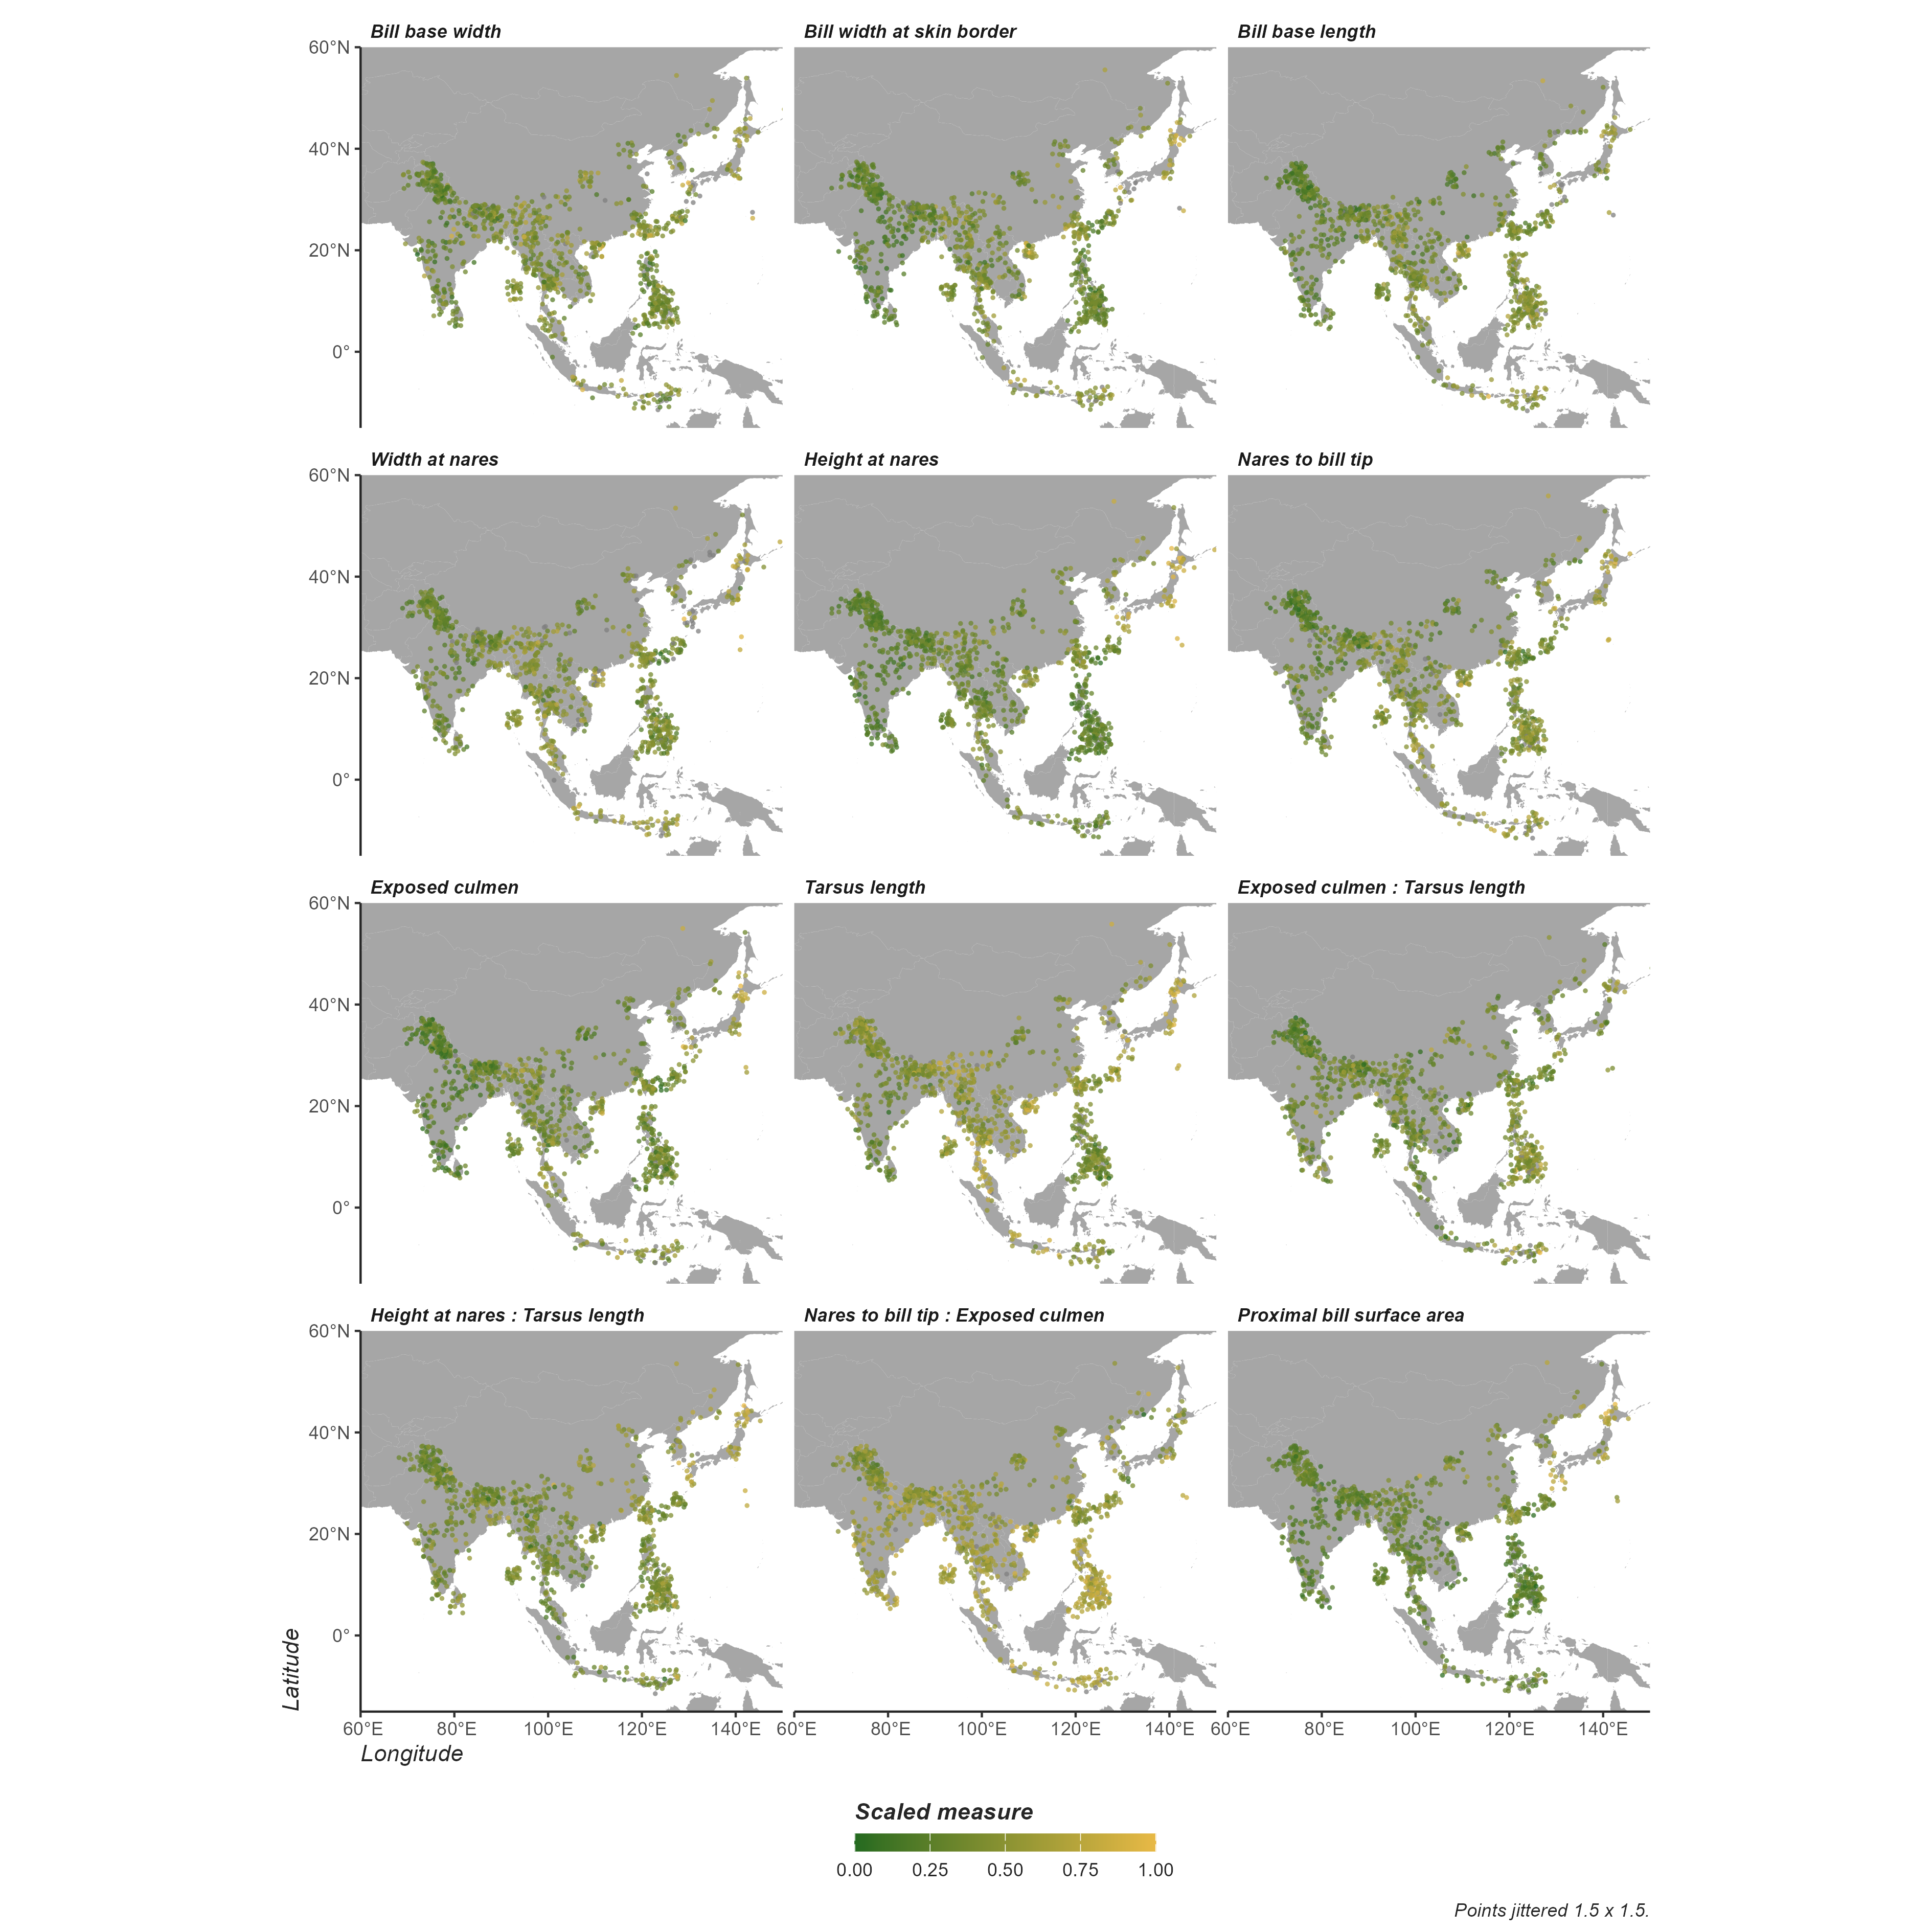
\includegraphics[width=0.9\linewidth]{../Figures/measuresMap} \caption{Scaled measures plotted to jittered locations (1.5x1.5).}\label{fig:measuresMap}
\end{figure}

\begin{figure}
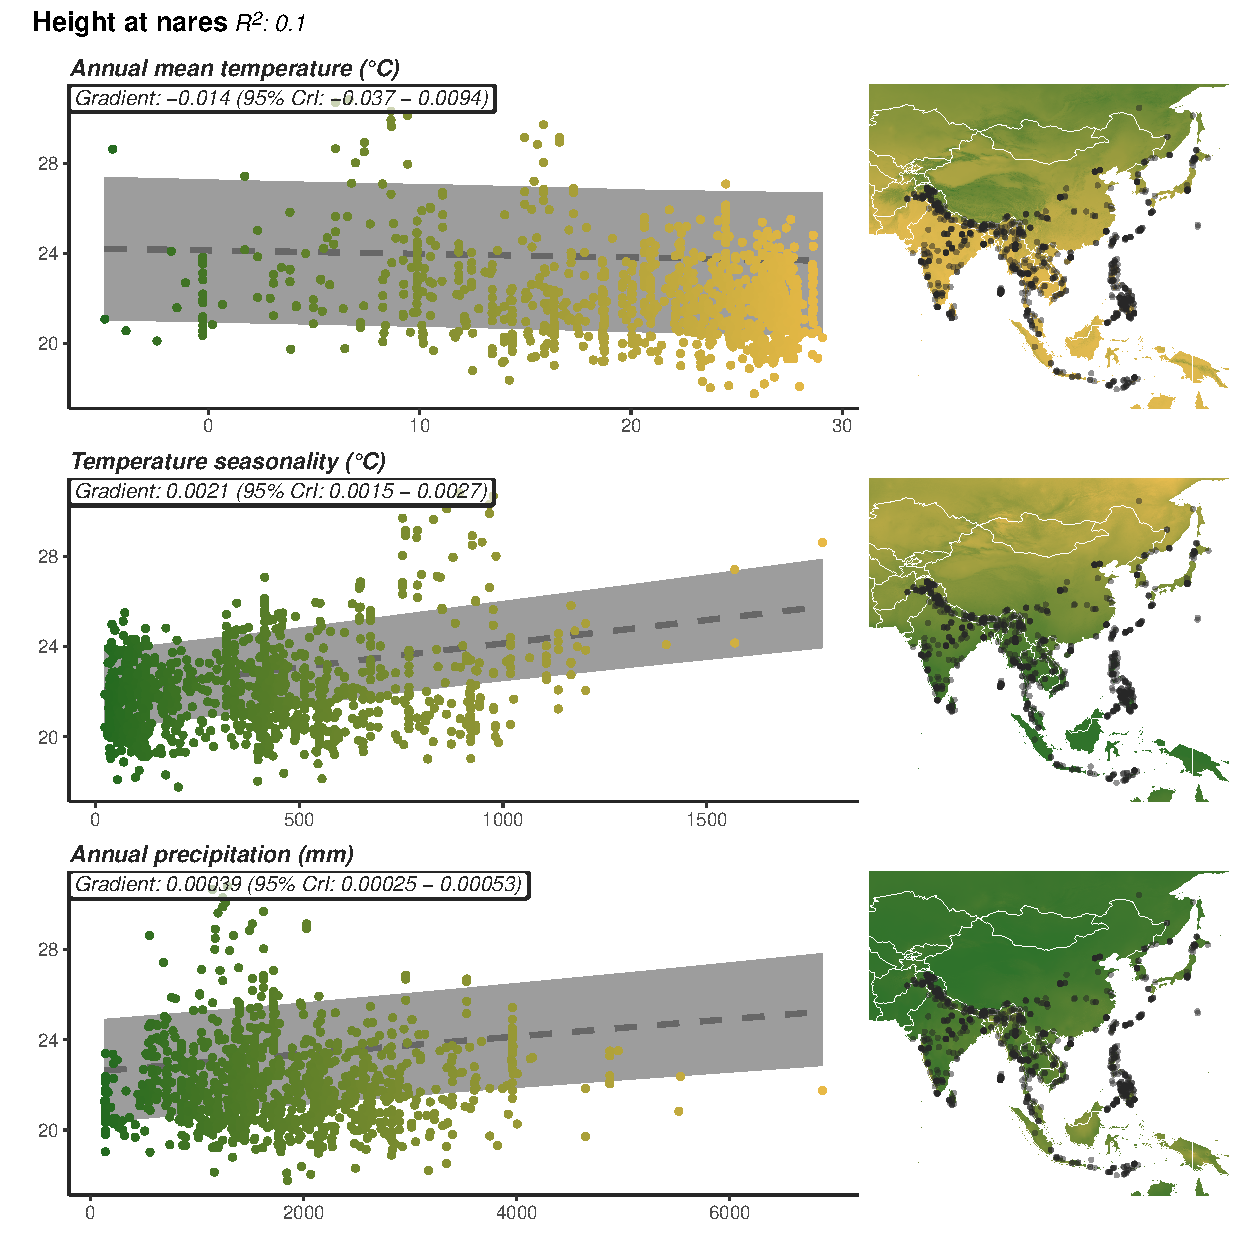
\includegraphics[width=0.9\linewidth]{../Figures/climMap_Height.at.nares} \caption{Measures of the Height at Nares in relation to annual mean temperature, temperature seasonality, and annual precipitation. Lower values are represented by dark green and higher values are represented by yellow.}\label{fig:climateComparisonMapHN}
\end{figure}

\begin{figure}
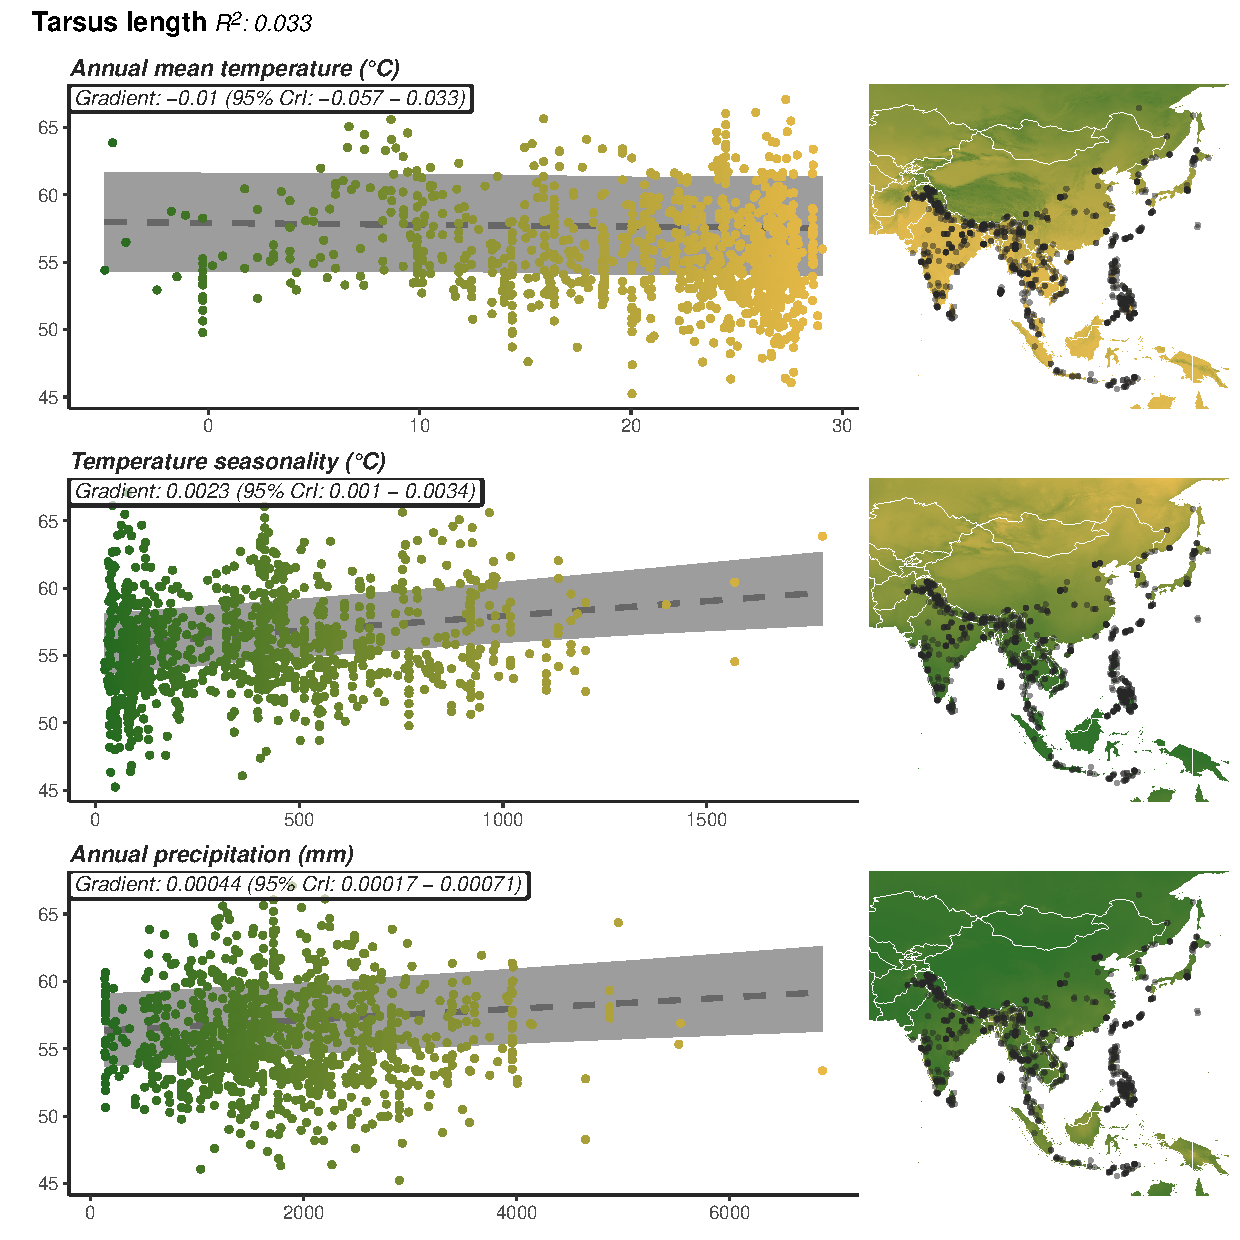
\includegraphics[width=0.9\linewidth]{../Figures/climMap_Tarsus.length} \caption{Measures of the Tarsus Length in relation to annual mean temperature, temperature seasonality, and annual precipitation. Lower values are represented by dark green and higher values are represented by yellow.}\label{fig:climateComparisonMapTL}
\end{figure}

\clearpage

\section*{References}\label{references}
\addcontentsline{toc}{section}{References}

\phantomsection\label{refs}
\begin{CSLReferences}{1}{0}
\bibitem[\citeproctext]{ref-acquarone_effects_2002}
Acquarone C, Cucco M, Cauli SL, Malacarne G. 2002. Effects of food abundance and predictability on body condition and health parameters: Experimental tests with the {Hooded} {Crow}. \emph{Ibis} 144. DOI: \href{https://doi.org/10.1046/j.1474-919X.2002.t01-2-00094_1.x}{10.1046/j.1474-919X.2002.t01-2-00094\_1.x}.

\bibitem[\citeproctext]{ref-alamshah2024morphological}
Alamshah A. 2024. The morphological and behavioral responses of jungle crows (corvus macrorhynchos) to environmental and human-induced changes. PhD thesis Thesis. State University of New York at Binghamton.

\bibitem[\citeproctext]{ref-alamshah_distribution-wide_2025}
Alamshah AL, Marshall BM. 2025. Distribution-wide morphometric data of {Jungle} {Crows} ({Corvus} macrorhynchos). \emph{Data in Brief}:111325. DOI: \href{https://doi.org/10.1016/j.dib.2025.111325}{10.1016/j.dib.2025.111325}.

\bibitem[\citeproctext]{ref-rmarkdown2024}
Allaire J, Xie Y, Dervieux C, McPherson J, Luraschi J, Ushey K, Atkins A, Wickham H, Cheng J, Chang W, Iannone R. 2024. \emph{\href{https://github.com/rstudio/rmarkdown}{{rmarkdown}: Dynamic documents for r}}.

\bibitem[\citeproctext]{ref-ashton_patterns_2002}
Ashton KG. 2002. Patterns of within‐species body size variation of birds: Strong evidence for {Bergmann}'s rule. \emph{Global Ecology and Biogeography} 11:505--523. DOI: \href{https://doi.org/10.1046/j.1466-822X.2002.00313.x}{10.1046/j.1466-822X.2002.00313.x}.

\bibitem[\citeproctext]{ref-babbitt_selection_2007}
Babbitt GA, Frederick PC. 2007. Selection for {Sexual} {Bill} {Dimorphism} in {Ibises}: {An} {Evaluation} of {Hypotheses}. \emph{Waterbirds} 30:199--206. DOI: \href{https://doi.org/10.1675/1524-4695(2007)30\%5B199:SFSBDI\%5D2.0.CO;2}{10.1675/1524-4695(2007)30{[}199:SFSBDI{]}2.0.CO;2}.

\bibitem[\citeproctext]{ref-badyaev_growing_2002}
Badyaev AV. 2002. Growing apart: An ontogenetic perspective on the evolution of sexual size dimorphism. \emph{Trends in Ecology \& Evolution} 17:369--378. DOI: \href{https://doi.org/10.1016/S0169-5347(02)02569-7}{10.1016/S0169-5347(02)02569-7}.

\bibitem[\citeproctext]{ref-bodawatta_ecological_2022}
Bodawatta KH, Shriner I, Pigott S, Koane B, Vinagre‐Izquierdo C, Rios RS, Jønsson KA, Tori WP. 2022. Ecological factors driving the feather mite associations in tropical avian hosts. \emph{Journal of Avian Biology} 2022:e02951. DOI: \href{https://doi.org/10.1111/jav.02951}{10.1111/jav.02951}.

\bibitem[\citeproctext]{ref-burkner_brms_2017}
Bürkner P-C. 2017a. Brms: {An} {R} {Package} for {Bayesian} {Multilevel} {Models} {Using} {Stan}. \emph{Journal of Statistical Software} 80:1--28. DOI: \href{https://doi.org/10.18637/jss.v080.i01}{10.18637/jss.v080.i01}.

\bibitem[\citeproctext]{ref-brms2017}
Bürkner P-C. 2017b. {brms}: An {R} package for {Bayesian} multilevel models using {Stan}. \emph{Journal of Statistical Software} 80:1--28. DOI: \href{https://doi.org/10.18637/jss.v080.i01}{10.18637/jss.v080.i01}.

\bibitem[\citeproctext]{ref-burkner_brms_2018}
Bürkner P-C. 2018a. Advanced {Bayesian} multilevel modeling with the {R} package {brms}. \emph{The R Journal} 10:395--411. DOI: \href{https://doi.org/10.32614/RJ-2018-017}{10.32614/RJ-2018-017}.

\bibitem[\citeproctext]{ref-brms2018}
Bürkner P-C. 2018b. Advanced {Bayesian} multilevel modeling with the {R} package {brms}. \emph{The R Journal} 10:395--411. DOI: \href{https://doi.org/10.32614/RJ-2018-017}{10.32614/RJ-2018-017}.

\bibitem[\citeproctext]{ref-burkner_brms_2021}
Bürkner P-C. 2021a. Bayesian item response modeling in {R} with {brms} and {Stan}. \emph{Journal of Statistical Software} 100:1--54. DOI: \href{https://doi.org/10.18637/jss.v100.i05}{10.18637/jss.v100.i05}.

\bibitem[\citeproctext]{ref-brms2021}
Bürkner P-C. 2021b. Bayesian item response modeling in {R} with {brms} and {Stan}. \emph{Journal of Statistical Software} 100:1--54. DOI: \href{https://doi.org/10.18637/jss.v100.i05}{10.18637/jss.v100.i05}.

\bibitem[\citeproctext]{ref-burton_geographical_2010}
Burton JA, Nietsch A. 2010. Geographical {Variation} in {Duet} {Songs} of {Sulawesi} {Tarsiers}: {Evidence} for {New} {Cryptic} {Species} in {South} and {Southeast} {Sulawesi}. \emph{International Journal of Primatology} 31:1123--1146. DOI: \href{https://doi.org/10.1007/s10764-010-9449-8}{10.1007/s10764-010-9449-8}.

\bibitem[\citeproctext]{ref-diblasi_phoretic_2018}
DiBlasi E, Johnson KP, Stringham SA, Hansen AN, Beach AB, Clayton DH, Bush SE. 2018. Phoretic dispersal influences parasite population genetic structure. \emph{Molecular Ecology} 27:2770--2779. DOI: \href{https://doi.org/10.1111/mec.14719}{10.1111/mec.14719}.

\bibitem[\citeproctext]{ref-dickinson_systematic_2004}
Dickinson EC, Eck S, Martens J. 2004. Systematic notes on {Asian} birds. 44. {A} preliminary review of the {Corvidae}. \emph{Zoologische Verhandelingen Leiden} 350:85--109.

\bibitem[\citeproctext]{ref-dube_microclimate_2018}
Dube WC, Hund AK, Turbek SP, Safran RJ. 2018. Microclimate and host body condition influence mite population growth in a wild bird-ectoparasite system. \emph{International Journal for Parasitology: Parasites and Wildlife} 7:301--308. DOI: \href{https://doi.org/10.1016/j.ijppaw.2018.07.007}{10.1016/j.ijppaw.2018.07.007}.

\bibitem[\citeproctext]{ref-dufresnes_speciation_2025}
Dufresnes C, Jablonski D, Ambu J, Prasad VK, Bala Gautam K, Kamei RG, Mahony S, Hofmann S, Masroor R, Alard B, Crottini A, Edmonds D, Ohler A, Jiang J, Khatiwada JR, Gupta SK, Borzée A, Borkin LJ, Skorinov DV, Melnikov DA, Milto KD, Konstantinov EL, Künzel S, Suchan T, Arkhipov DV, Trofimets AV, Nguyen TV, Suwannapoom C, Litvinchuk SN, Poyarkov NA. 2025. Speciation and historical invasions of the {Asian} black-spined toad ({Duttaphrynus} melanostictus). \emph{Nature Communications} 16. DOI: \href{https://doi.org/10.1038/s41467-024-54933-4}{10.1038/s41467-024-54933-4}.

\bibitem[\citeproctext]{ref-garg_genome-wide_2016}
Garg KM, Tizard R, Ng NSR, Cros E, Dejtaradol A, Chattopadhyay B, Pwint N, Päckert M, Rheindt FE. 2016. Genome-wide data help identify an avian species-level lineage that is morphologically and vocally cryptic. \emph{Molecular Phylogenetics and Evolution} 102:97--103. DOI: \href{https://doi.org/10.1016/j.ympev.2016.05.028}{10.1016/j.ympev.2016.05.028}.

\bibitem[\citeproctext]{ref-geist_nasal_2000}
Geist NR. 2000. Nasal {Respiratory} {Turbinate} {Function} in {Birds}. \emph{Physiological and Biochemical Zoology} 73:581--589. DOI: \href{https://doi.org/10.1086/317750}{10.1086/317750}.

\bibitem[\citeproctext]{ref-gwee_species_2019}
Gwee CY, Eaton JA, Ng EYX, Rheindt FE. 2019. Species delimitation within the {Glaucidium} brodiei owlet complex using bioacoustic tools. \emph{Avian Research} 10:36. DOI: \href{https://doi.org/10.1186/s40657-019-0175-4}{10.1186/s40657-019-0175-4}.

\bibitem[\citeproctext]{ref-Metrics}
Hamner B, Frasco M. 2018. \emph{\href{https://CRAN.R-project.org/package=Metrics}{{Metrics}: Evaluation metrics for machine learning}}.

\bibitem[\citeproctext]{ref-hartert_types_1922}
Hartert E, Zoological Museum (Tring, England). 1922. \emph{Types of birds in the {Tring} {Museum}}. n. p: {[}s.n.{]}. DOI: \href{https://doi.org/10.5962/bhl.title.57071}{10.5962/bhl.title.57071}.

\bibitem[\citeproctext]{ref-heiss_growth_2009}
Heiss RS, Clark AB, McGowan KJ. 2009. Growth and nutritional state of {American} {Crow} nestlings vary between urban and rural habitats. \emph{Ecological Applications} 19:829--839. DOI: \href{https://doi.org/10.1890/08-0140.1}{10.1890/08-0140.1}.

\bibitem[\citeproctext]{ref-tidyselect}
Henry L, Wickham H. 2024. \emph{\href{https://CRAN.R-project.org/package=tidyselect}{{tidyselect}: Select from a set of strings}}.

\bibitem[\citeproctext]{ref-glue}
Hester J, Bryan J. 2024. \emph{\href{https://CRAN.R-project.org/package=glue}{{glue}: Interpreted string literals}}.

\bibitem[\citeproctext]{ref-terra}
Hijmans RJ. 2025. \emph{\href{https://CRAN.R-project.org/package=terra}{{terra}: Spatial data analysis}}.

\bibitem[\citeproctext]{ref-huey_behavioral_2003}
Huey RB, Hertz PE, Sinervo B. 2003. Behavioral {Drive} versus {Behavioral} {Inertia} in {Evolution}: {A} {Null} {Model} {Approach}. \emph{The American Naturalist} 161:357--366. DOI: \href{https://doi.org/10.1086/346135}{10.1086/346135}.

\bibitem[\citeproctext]{ref-iucn_corvus_2016}
IUCN. 2016. Corvus macrorhynchos: {BirdLife} {International}: {The} {IUCN} {Red} {List} of {Threatened} {Species} 2016: E.{T103727590A94046488}. DOI: \href{https://doi.org/10.2305/IUCN.UK.2016-3.RLTS.T103727590A94046488.en}{10.2305/IUCN.UK.2016-3.RLTS.T103727590A94046488.en}.

\bibitem[\citeproctext]{ref-jones_age-related_2002}
Jones J, Francis CM, Drew M, Fuller S, Ng MWS. 2002. Age-{Related} {Differences} in {Body} {Mass} and {Rates} of {Mass} {Gain} of {Passerines} {During} {Autumn} {Migratory} {Stopover}. \emph{The Condor} 104:49--58. DOI: \href{https://doi.org/10.1093/condor/104.1.49}{10.1093/condor/104.1.49}.

\bibitem[\citeproctext]{ref-jonsson_brains_2012}
Jønsson KA, Fabre P-H, Irestedt M. 2012. Brains, tools, innovation and biogeography in crows and ravens. \emph{BMC Evolutionary Biology} 12:72. DOI: \href{https://doi.org/10.1186/1471-2148-12-72}{10.1186/1471-2148-12-72}.

\bibitem[\citeproctext]{ref-ggpubr}
Kassambara A. 2023. \emph{\href{https://CRAN.R-project.org/package=ggpubr}{{ggpubr}: {``{ggplot2}''} based publication ready plots}}.

\bibitem[\citeproctext]{ref-ggdist2024a}
Kay M. 2024a. {ggdist}: Visualizations of distributions and uncertainty in the grammar of graphics. \emph{IEEE Transactions on Visualization and Computer Graphics} 30:414--424. DOI: \href{https://doi.org/10.1109/TVCG.2023.3327195}{10.1109/TVCG.2023.3327195}.

\bibitem[\citeproctext]{ref-ggdist2024b}
Kay M. 2024b. \emph{{ggdist}: Visualizations of distributions and uncertainty}. DOI: \href{https://doi.org/10.5281/zenodo.3879620}{10.5281/zenodo.3879620}.

\bibitem[\citeproctext]{ref-tidybayes}
Kay M. 2024c. \emph{{tidybayes}: Tidy data and geoms for {Bayesian} models}. DOI: \href{https://doi.org/10.5281/zenodo.1308151}{10.5281/zenodo.1308151}.

\bibitem[\citeproctext]{ref-klockenhoff_zur_1969}
Klockenhoff H. 1969. Zur {Verbreitung} der {Mallophagen} der {Gattung} {Myrsidea} {Waterston} auf der {Dschungelkrähe} {Corvus} macrorhynchos {Wagler}. \emph{Journal of Zoological Systematics and Evolutionary Research} 7:53--58. DOI: \href{https://doi.org/10.1111/j.1439-0469.1969.tb00847.x}{10.1111/j.1439-0469.1969.tb00847.x}.

\bibitem[\citeproctext]{ref-tarchetypes}
Landau WM. 2021a. \emph{{tarchetypes}: Archetypes for targets}.

\bibitem[\citeproctext]{ref-targets}
Landau WM. 2021b. \href{https://doi.org/10.21105/joss.02959}{The targets r package: A dynamic make-like function-oriented pipeline toolkit for reproducibility and high-performance computing}. \emph{Journal of Open Source Software} 6:2959.

\bibitem[\citeproctext]{ref-crew}
Landau WM. 2024. \emph{\href{https://CRAN.R-project.org/package=crew}{{crew}: A distributed worker launcher framework}}.

\bibitem[\citeproctext]{ref-performance}
Lüdecke D, Ben-Shachar MS, Patil I, Waggoner P, Makowski D. 2021. {performance}: An {R} package for assessment, comparison and testing of statistical models. \emph{Journal of Open Source Software} 6:3139. DOI: \href{https://doi.org/10.21105/joss.03139}{10.21105/joss.03139}.

\bibitem[\citeproctext]{ref-billerman_large-billed_2020}
Madge S. 2020. Large-billed {Crow} ({Corvus} macrorhynchos). In: Billerman SM, Keeney BK, Rodewald PG, Schulenberg TS eds. \emph{Birds of the {World}}. Cornell Lab of Ornithology,. DOI: \href{https://doi.org/10.2173/bow.labcro1.01}{10.2173/bow.labcro1.01}.

\bibitem[\citeproctext]{ref-madge_crows_1999}
Madge S, Burn H. 1999. \emph{Crows and jays: A guide to the crows, jays and magpies of the world}. London: C. Helm.

\bibitem[\citeproctext]{ref-madge_crows_2010}
Madge S, Burn H. 2010. \emph{Crows and {Jays}: {Helm} {Identification} {Guides}}. A\&C Black.

\bibitem[\citeproctext]{ref-martens_calls_2000}
Martens J. 2000. Calls of the {Jungle} {Crow} ({Corvus} macrorhynchos s. L.) as a taxonomic {characterResults} of the {Himalaya} {Expeditions} of {J}. {Martens}, {No}. 224. - {For} {No}. 225 see: {Stuttgarter} {Beitr}. {Naturk}. {A598}, 1999. \emph{Journal für Ornithologie} 141:275. DOI: \href{https://doi.org/10.1046/j.1439-0361.2000.00026.x}{10.1046/j.1439-0361.2000.00026.x}.

\bibitem[\citeproctext]{ref-martens_towards_1995}
Martens J, Eck S. 1995. Towards an {Ornithology} of the {Himalayas}: {Systematics}, {Ecology}, and {Vocalizations} of {Nepal} {Birds}. \emph{Bonner zoologische Monographien} 38:375--390.

\bibitem[\citeproctext]{ref-here}
Müller K. 2020. \emph{\href{https://CRAN.R-project.org/package=here}{{here}: A simpler way to find your files}}.

\bibitem[\citeproctext]{ref-nakamura_postglacial_2016}
Nakamura S, Kryukov A. 2016. Postglacial colonisation and diversification of the {Jungle} {Crow} ({Corvus} macrorhynchos) in its north-eastern frontier as revealed by morphological analysis. \emph{Journal of Ornithology} 157:1087--1101. DOI: \href{https://doi.org/10.1007/s10336-016-1356-0}{10.1007/s10336-016-1356-0}.

\bibitem[\citeproctext]{ref-noce_cmcc-bioclimind_2019}
Noce S, Caporaso L, Santini M. 2019. {CMCC}-{BioClimInd}. {A} new globaldataset of bioclimatic indicators. DOI: \href{https://doi.org/10.1594/PANGAEA.904278}{10.1594/PANGAEA.904278}.

\bibitem[\citeproctext]{ref-noce_new_2020}
Noce S, Caporaso L, Santini M. 2020. A new global dataset of bioclimatic indicators. \emph{Scientific Data} 7:398. DOI: \href{https://doi.org/10.1038/s41597-020-00726-5}{10.1038/s41597-020-00726-5}.

\bibitem[\citeproctext]{ref-olsson_non-monophyletic_2005}
Olsson U, Alström P, Ericson PGP, Sundberg P. 2005. Non-monophyletic taxa and cryptic species---{Evidence} from a molecular phylogeny of leaf-warblers ({Phylloscopus}, {Aves}). \emph{Molecular Phylogenetics and Evolution} 36:261--276. DOI: \href{https://doi.org/10.1016/j.ympev.2005.01.012}{10.1016/j.ympev.2005.01.012}.

\bibitem[\citeproctext]{ref-outlaw_pliocene_2008}
Outlaw DC, Voelker G. 2008. Pliocene climatic change in insular {Southeast} {Asia} as an engine of diversification in \emph{ficedula} flycatchers. \emph{Journal of Biogeography} 35:739--752. DOI: \href{https://doi.org/10.1111/j.1365-2699.2007.01821.x}{10.1111/j.1365-2699.2007.01821.x}.

\bibitem[\citeproctext]{ref-owens_sexual_1998}
Owens IPF, Hartley IR. 1998. Sexual dimorphism in birds: Why are there so many different forms of dimorphism? \emph{Proceedings of the Royal Society of London. Series B: Biological Sciences} 265:397--407. DOI: \href{https://doi.org/10.1098/rspb.1998.0308}{10.1098/rspb.1998.0308}.

\bibitem[\citeproctext]{ref-patchwork}
Pedersen TL. 2024. \emph{\href{https://CRAN.R-project.org/package=patchwork}{{patchwork}: The composer of plots}}.

\bibitem[\citeproctext]{ref-pfenninger_cryptic_2007}
Pfenninger M, Schwenk K. 2007. Cryptic animal species are homogeneously distributed among taxa and biogeographical regions. \emph{BMC Evolutionary Biology} 7:121. DOI: \href{https://doi.org/10.1186/1471-2148-7-121}{10.1186/1471-2148-7-121}.

\bibitem[\citeproctext]{ref-pierce_diet_2004}
Pierce BJ, McWilliams SR. 2004. Diet {Quality} and {Food} {Limitation} {Affect} the {Dynamics} of {Body} {Composition} and {Digestive} {Organs} in a {Migratory} {Songbird} ( \emph{{Zonotrichia} albicollis} ). \emph{Physiological and Biochemical Zoology} 77:471--483. DOI: \href{https://doi.org/10.1086/383503}{10.1086/383503}.

\bibitem[\citeproctext]{ref-rstudio}
Posit team. 2024. \emph{\href{http://www.posit.co/}{{RStudio}: Integrated development environment for r}}. Boston, MA: Posit Software, PBC.

\bibitem[\citeproctext]{ref-probst_effects_2022}
Probst CM, Ralston J, Bentley I. 2022. Effects of climate on bill morphology within and across \emph{toxostoma} thrashers. \emph{Journal of Avian Biology} 2022:jav.02871. DOI: \href{https://doi.org/10.1111/jav.02871}{10.1111/jav.02871}.

\bibitem[\citeproctext]{ref-QGIS_software}
QGIS Development Team. 2024. \emph{\href{https://www.qgis.org}{QGIS geographic information system}}. QGIS Association.

\bibitem[\citeproctext]{ref-base}
R Core Team. 2024. \emph{\href{https://www.R-project.org/}{{R}: A language and environment for statistical computing}}. Vienna, Austria: R Foundation for Statistical Computing.

\bibitem[\citeproctext]{ref-reid_impact_2024}
Reid R, Capilla-Lasheras P, Haddou Y, Boonekamp J, Dominoni DM. 2024. The impact of urbanization on health depends on the health metric, life stage and level of urbanization: A global meta-analysis on avian species. \emph{Proceedings of the Royal Society B: Biological Sciences} 291:20240617. DOI: \href{https://doi.org/10.1098/rspb.2024.0617}{10.1098/rspb.2024.0617}.

\bibitem[\citeproctext]{ref-rutz_evolutionary_2012}
Rutz C, St Clair JJH. 2012. The evolutionary origins and ecological context of tool use in {New} {Caledonian} crows. \emph{Behavioural Processes} 89:153--165. DOI: \href{https://doi.org/10.1016/j.beproc.2011.11.005}{10.1016/j.beproc.2011.11.005}.

\bibitem[\citeproctext]{ref-schneider_nih_2012}
Schneider CA, Rasband WS, Eliceiri KW. 2012. {NIH} {Image} to {ImageJ}: 25 years of image analysis. \emph{Nature Methods} 9:671--675. DOI: \href{https://doi.org/10.1038/nmeth.2089}{10.1038/nmeth.2089}.

\bibitem[\citeproctext]{ref-senar_keel_1997}
Senar JC, Pascual J. 1997. Keel and tarsus length may provide a good predictor of avian body size. \emph{Ardea} 85:269--274.

\bibitem[\citeproctext]{ref-shankar_king_2021}
Shankar PG, Swamy P, Williams RC, Ganesh SR, Moss M, Höglund J, Das I, Sahoo G, Vijayakumar SP, Shanker K, Wüster W, Dutta SK. 2021. King or royal family? {Testing} for species boundaries in the {King} {Cobra}, {Ophiophagus} hannah ({Cantor}, 1836), using morphology and multilocus {DNA} analyses. \emph{Molecular Phylogenetics and Evolution}:107300. DOI: \href{https://doi.org/10.1016/j.ympev.2021.107300}{10.1016/j.ympev.2021.107300}.

\bibitem[\citeproctext]{ref-singh_taxonomy_2020}
Singh A, Gupta SK, Alström P, Mohan D, Hooper DM, Kumar RS, Bhatt D, Singh P, Price TD. 2020. Taxonomy of cryptic species in the {Cyornis} rubeculoides complex in the {Indian} subcontinent. \emph{Ibis} 162:924--935. DOI: \url{https://doi.org/10.1111/ibi.12735}.

\bibitem[\citeproctext]{ref-sol_behavioural_2002}
Sol D, Timmermans S, Lefebvre L. 2002. Behavioural flexibility and invasion success in birds. \emph{Animal Behaviour} 63:495--502. DOI: \href{https://doi.org/10.1006/anbe.2001.1953}{10.1006/anbe.2001.1953}.

\bibitem[\citeproctext]{ref-sweet_role_2018}
Sweet AD, Johnson KP. 2018. The role of parasite dispersal in shaping a host--parasite system at multiple evolutionary scales. \emph{Molecular Ecology} 27:5104--5119. DOI: \href{https://doi.org/10.1111/mec.14937}{10.1111/mec.14937}.

\bibitem[\citeproctext]{ref-tattersall_heat_2009}
Tattersall GJ, Andrade DV, Abe AS. 2009. Heat {Exchange} from the {Toucan} {Bill} {Reveals} a {Controllable} {Vascular} {Thermal} {Radiator}. \emph{Science} 325:468--470. DOI: \href{https://doi.org/10.1126/science.1175553}{10.1126/science.1175553}.

\bibitem[\citeproctext]{ref-tobias_avonet_2022}
Tobias JA, Sheard C, Pigot AL, Devenish AJM, Yang J, Sayol F, Neate‐Clegg MHC, Alioravainen N, Weeks TL, Barber RA, Walkden PA, MacGregor HEA, Jones SEI, Vincent C, Phillips AG, Marples NM, Montaño‐Centellas FA, Leandro‐Silva V, Claramunt S, Darski B, Freeman BG, Bregman TP, Cooney CR, Hughes EC, Capp EJR, Varley ZK, Friedman NR, Korntheuer H, Corrales‐Vargas A, Trisos CH, Weeks BC, Hanz DM, Töpfer T, Bravo GA, Remeš V, Nowak L, Carneiro LS, Moncada R. AJ, Matysioková B, Baldassarre DT, Martínez‐Salinas A, Wolfe JD, Chapman PM, Daly BG, Sorensen MC, Neu A, Ford MA, Mayhew RJ, Fabio Silveira L, Kelly DJ, Annorbah NND, Pollock HS, Grabowska‐Zhang AM, McEntee JP, Carlos T. Gonzalez J, Meneses CG, Muñoz MC, Powell LL, Jamie GA, Matthews TJ, Johnson O, Brito GRR, Zyskowski K, Crates R, Harvey MG, Jurado Zevallos M, Hosner PA, Bradfer‐Lawrence T, Maley JM, Stiles FG, Lima HS, Provost KL, Chibesa M, Mashao M, Howard JT, Mlamba E, Chua MAH, Li B, Gómez MI, García NC, Päckert M, Fuchs J, Ali JR, Derryberry EP, Carlson ML, Urriza RC, Brzeski KE, Prawiradilaga DM, Rayner MJ, Miller ET, Bowie RCK, Lafontaine R, Scofield RP, Lou Y, Somarathna L, Lepage D, Illif M, Neuschulz EL, Templin M, Dehling DM, Cooper JC, Pauwels OSG, Analuddin K, Fjeldså J, Seddon N, Sweet PR, DeClerck FAJ, Naka LN, Brawn JD, Aleixo A, Böhning‐Gaese K, Rahbek C, Fritz SA, Thomas GH, Schleuning M. 2022. {AVONET}: Morphological, ecological and geographical data for all birds. \emph{Ecology Letters} 25:581--597. DOI: \href{https://doi.org/10.1111/ele.13898}{10.1111/ele.13898}.

\bibitem[\citeproctext]{ref-troscianko_extreme_2012}
Troscianko J, Von Bayern AMPP, Chappell J, Rutz C, Martin GR. 2012. Extreme binocular vision and a straight bill facilitate tool use in {New} {Caledonian} crows. \emph{Nature Communications} 3:1110. DOI: \href{https://doi.org/10.1038/ncomms2111}{10.1038/ncomms2111}.

\bibitem[\citeproctext]{ref-voda_cryptic_2015}
Vodă R, Dapporto L, Dincă V, Vila R. 2015. Cryptic matters: Overlooked species generate most butterfly beta‐diversity. \emph{Ecography} 38:405--409. DOI: \href{https://doi.org/10.1111/ecog.00762}{10.1111/ecog.00762}.

\bibitem[\citeproctext]{ref-whistler_popular_2008}
Whistler H. 2008. Popular {Handbook} of {Indian} {Birds}. \emph{Ibis} 84:449--450. DOI: \href{https://doi.org/10.1111/j.1474-919X.1942.tb05725.x}{10.1111/j.1474-919X.1942.tb05725.x}.

\bibitem[\citeproctext]{ref-tidyverse}
Wickham H, Averick M, Bryan J, Chang W, McGowan LD, François R, Grolemund G, Hayes A, Henry L, Hester J, Kuhn M, Pedersen TL, Miller E, Bache SM, Müller K, Ooms J, Robinson D, Seidel DP, Spinu V, Takahashi K, Vaughan D, Wilke C, Woo K, Yutani H. 2019. Welcome to the {tidyverse}. \emph{Journal of Open Source Software} 4:1686. DOI: \href{https://doi.org/10.21105/joss.01686}{10.21105/joss.01686}.

\bibitem[\citeproctext]{ref-williams_photography_2020}
Williams HM, Wilcox SB, Patterson AJ. 2020. Photography as a tool for avian morphometric measurements. \emph{Journal of Ornithology} 161:333--339. DOI: \href{https://doi.org/10.1007/s10336-019-01728-w}{10.1007/s10336-019-01728-w}.

\bibitem[\citeproctext]{ref-wyles_birds_1983}
Wyles JS, Kunkel JG, Wilson AC. 1983. Birds, behavior, and anatomical evolution. \emph{Proceedings of the National Academy of Sciences} 80:4394--4397. DOI: \href{https://doi.org/10.1073/pnas.80.14.4394}{10.1073/pnas.80.14.4394}.

\bibitem[\citeproctext]{ref-knitr2014}
Xie Y. 2014. {knitr}: A comprehensive tool for reproducible research in {R}. In: Stodden V, Leisch F, Peng RD eds. \emph{Implementing reproducible computational research}. Chapman; Hall/CRC,.

\bibitem[\citeproctext]{ref-knitr2015}
Xie Y. 2015. \emph{\href{https://yihui.org/knitr/}{Dynamic documents with {R} and knitr}}. Boca Raton, Florida: Chapman; Hall/CRC.

\bibitem[\citeproctext]{ref-bookdown2016}
Xie Y. 2016. \emph{\href{https://bookdown.org/yihui/bookdown}{{bookdown}: Authoring books and technical documents with {R} markdown}}. Boca Raton, Florida: Chapman; Hall/CRC.

\bibitem[\citeproctext]{ref-knitr2024}
Xie Y. 2024. \emph{\href{https://yihui.org/knitr/}{{knitr}: A general-purpose package for dynamic report generation in r}}.

\bibitem[\citeproctext]{ref-bookdown2025}
Xie Y. 2025. \emph{\href{https://github.com/rstudio/bookdown}{{bookdown}: Authoring books and technical documents with r markdown}}.

\bibitem[\citeproctext]{ref-rmarkdown2018}
Xie Y, Allaire JJ, Grolemund G. 2018. \emph{\href{https://bookdown.org/yihui/rmarkdown}{R markdown: The definitive guide}}. Boca Raton, Florida: Chapman; Hall/CRC.

\bibitem[\citeproctext]{ref-rmarkdown2020}
Xie Y, Dervieux C, Riederer E. 2020. \emph{\href{https://bookdown.org/yihui/rmarkdown-cookbook}{R markdown cookbook}}. Boca Raton, Florida: Chapman; Hall/CRC.

\end{CSLReferences}

\end{document}
